%%%%%%%%%%%%%%%%%%%%%%%%%%%%%%%%%%%%%%%%%%%%%%%%%%%%%%%%%%%%%%%%%%%%%%%%
%                                                                      %
%     File: Thesis_Implementation.tex                                  %
%     Tex Master: Thesis.tex                                           %
%                                                                      %
%     Author: Andre C. Marta                                           %
%     Last modified :  2 Jul 2015                                      %
%                                                                      %
%%%%%%%%%%%%%%%%%%%%%%%%%%%%%%%%%%%%%%%%%%%%%%%%%%%%%%%%%%%%%%%%%%%%%%%%

\chapter{Monografia:Sialoadenose responsiva a fenobarbital}
\label{chapter:Monografia:Sialoadenose responsiva a fenobarbital}

Insert your chapter material here... CARLOS TU ES MUITO BOM, AMO-TE
Es o mais lindo do mundo 
%%%%%%%%%%%%%%%%%%%%%%%%%%%%%%%%%%%%%%%%%%%%%%%%%%%%%%%%%%%%%%%%%%%%%%%%
\section{Introdução ao tema}
\label{section:Introdução ao tema}

Description of the numerical implementation of the models explained in Chapter

%%%%%%%%%%%%%%%%%%%%%%%%%%%%%%%%%%%%%%%%%%%%%%%%%%%%%%%%%%%%%%%%%%%%%%%%
\section{Glândulas salivares}
\label{section:Glândulas salivares}

\subsection{Anatomia e Fisiologia das glândulas salivares}

As glândulas salivares são glândulas exócrinas pares localizadas na cavidade oral, cuja principal função é a produção de saliva. \cite{Mescher2018}Estas glândulas integram-se funcionalmente no sistema digestivo, a par do pâncreas, fígado e vesícula biliar. \cite{Mescher2018} Produtos produzidos por estes órgãos auxiliam e facilitam o transporte e digestão do alimento ao longo do trato gastrointestinal. \cite{Mescher2018}

Anatomicamente, são glândulas lobuladas, compostas por ácinos e respetivos ductos excretores, funcionalmente distintos. Cada ácino é circunscrito por células glandulares epiteliais, que segregam uma mistura de água, eletrólitos, enzimas e muco para o lúmen acinar. \cite{Proctor2007,cunningham} Os ácinos classificam-se em serosos (ricos em grânulos de zimogénio), mucosos ou mistos/seromucosos.\cite{cunningham} Neste último tipo, frequentemente observa-se a presença de semiluas serosas, onde grupos de células serosas se localizam perifericamente a ácinos mucosos.\cite{Das_Textbook,cunningham} 

À medida que a saliva percorre os ductos coletores, a sua composição é alterada. \cite{Proctor2007,cunningham} O epitélio do ducto reabsorve eletrólitos, nomeadamente sódio e cloreto, resultando num produto final hipotónico, com concentração inferior à do fluido extracelular. Esta modificação é tanto menor quanto maior for a taxa de secreção, o que se traduz numa saliva com maior tonicidade e conteúdo eletrolítico em situações de estímulo aumentado. \cite{cunningham} 

Rodeando os ácinos e ductos proximais encontram-se células mioepiteliais, especializadas, com características de músculo liso modificado.\cite{cunningham} Estas células, também designadas por "células em cesto" devido à morfologia do seu citoplasma ramificado, contraem-se promovendo o aumento da pressão intraductal, facilitando assim a ejeção da saliva. \cite{Das_Textbook,cunningham}

\subsubsection{Classificação e localização das glândulas salivares em cães}

As glândulas salivares estão agrupadas em:
\begin{enumerate}
    \item	Glândulas salivares menores;
    \item Glândulas salivares maiores.
\end{enumerate}

As glândulas salivares menores distribuem-se pela mucosa dos lábios, bochechas, língua, palato mole, soalho sublingual, faringe e esófago. \cite{Singh2017} Embora individualmente tenham pouca expressão funcional, a sua contribuição coletiva é significativa,\cite{Singh2017} sendo responsáveis por uma secreção contínua, lenta e espontânea, que desempenha um papel crucial na manutenção da humidade da cavidade oral. \cite{Cappai2021}

As glândulas salivares maiores, por sua vez, são as principais responsáveis pela produção e excreção de saliva para a cavidade oral, estando ligadas a esta através de ductos secretores. \cite{Singh2017},VeterinayAnatomy VET HISTOLOGY 

Este grupo inclui as glândulas parótida, mandibular, zigomática e sublingual, sendo esta última dividida nas porções monostomática e polistomática.VET HISTOLOGY Todas estas glândulas estão envolvidas por uma cápsula de tecido conjuntivo designada por \textit{capsula glandularis}.VET HISTOLOGY

\subsubsection{Glândula parótida}

A glândula parótida, cujo nome deriva do latim \textit{glândula parotis}, localiza-se na junção entre a cabeça e o pescoço, sobrejacente  à base da cartilagem auricular. Trata-se de uma estrutura relativamente pequena e confinada à região auricular, com um contorno em V, cujo ápex se orienta ventralmente.\cite{Singh2017}

Anatomicamente, está delimitada caudalmente pela parte mastoide do músculo esternocefálico e pela parte cervical do cleidocefálico, e rostralmente pelo músculo masséter e articulação temporomandibular.\cite{Singh2017} Apresenta um peso médio de 7 g e dimensões aproximadas de 6 x 1,5 cm.\cite{Singh2017}
A glândula divide-se em duas porções: superficial (pars superficialis), constituída por dois ramos em V unidos por uma porção fina, e profunda (pars profunda), com morfologia em cunha, localizada ventralmente à cartilagem do meato acústico externo.\cite{Singh2017} Esta última estende-se medialmente até à bula timpânica e à parede da nasofaringe, posicionando-se dorsalmente ao polo rostral da glândula mandibular.\cite{Singh2017}
Os seus três ângulos projetam-se em direções dorso-rostral, dorso-caudal e ventral, enquanto as bordas são dorsal, rostral e caudal.\cite{Singh2017} A superfície superficial  é quase plana no sentido transversal e ligeiramente convexa no sentido longitudinal.\cite{Singh2017} Esta superfície é atravessada verticalmente pelo músculo parotídeo auricular (\textit{m. parotidoauricularis} , anteriormente designado\textit{m. depressor auriculae} ), que, por sua vez, é parcialmente coberto por fascículos do músculo platisma.\cite{Singh2017} A veia maxilar atravessa a glândula junto ao seu ângulo ventral.\cite{Singh2017}


Do bordo rostral emergem, da zona mais profunda, os ramos plapebral, auriculotemporal e os ramos bucais dorsal e ventral do nervo facial, bem como a artéria e veia auricular rostral e a artéria facial transversa.\cite{Singh2017} O linfonodo parotídeo encontra-se, na maioria dos casos, medialmente ao bordo rostral da porção superficial da glândula.\cite{Singh2017} O bordo caudal é circunscrito por ramos dos vasos auriculares intermédios que podem até atravessar a glândula.\cite{Singh2017}
O bordo dorsal não se encontra próximo de nervos e vasos sanguíneos relevantes, no entanto, há uma relação de proximidade com a cartilagem do meato acústico externo.\cite{Singh2017} Em cirurgias otológicas, como na remoção da parede lateral da cartilagem auricular em casos de otite externa crónica, é essencial proceder ao deslocamento ventral da glândula, a fim de prevenir lesões iatrogénicas. \cite{Singh2017}


A porção profunda caudal está intimamente relacionada com o nervo facial e os seus ramos terminais.\cite{Singh2017} A porção rostral profunda está também relacionada com o nervo maxilar e com as artérias temporais superficiais.\cite{Singh2017}
O ducto parotídeo, com cerca de 1,5 mm  de diâmetro e 6 cms de comprimento, origina-se da confluência de duas a três raízes emergentes do terço ventral do bordo rostral da glândula.\cite{Singh2017} Este ducto percorre a superfície lateral do músculo masséter, ao qual está aderido por fáscia superficial, drigindo-se paralelamente às fibras musculares até atingir a mucosa jugal.\cite{Singh2017} Termina ao nível da extremidade rostral de uma crista mucosa discreta, situada na margem caudal do quarto pré-molar superior, junto ao fórnix formado pela junção da bochecha com a maxila.\cite{Singh2017}


A irrigação arterial é assegurada maioritariamente pela artéria parotídea, ramo da carótida externa, com contribuição adicional das artérias auricular caudal, facial transversa e auricular rostral.\cite{Singh2017} A drenagem venosa é feita por tributárias das veias temporal superficial e auricular caudal.\cite{Singh2017}


A drenagem linfática é efetuada para os gânglios linfáticos parotídeos e retrofaríngeos mediais.\cite{Singh2017}


A inervação parassimpática é mediada pelo nervo auriculotemporal, ramo do nervo mandibular.\cite{Singh2017} Os corpos celulares dos neurónios pré ganglionares localizam-se no núcleo salivar inferior do nervo glossofaríngeo (IX par craniano), na medula oblonga.\cite{Singh2017} Os axónios percorrem o nervo IX, formando o plexo timpânico, seguem pelo nervo petroso menor até ao gânglio ótico, onde ocorre a sinapse com os neurónios pós ganglionares. Estes prosseguem pelo nervo auriculotemporal até à glândula.\cite{Singh2017}


A inervação simpática é composta por fibras pós ganglionares oriundas do gânglio cervical cranial, que acompanham as artérias aferentes à glândula.\cite{Singh2017}

\subsubsection{Glândula mandibular}

A glândula mandibular é uma estrutura ovoide \cite{evans_millers_2012}\cite{Singh2017}localizada caudalmente ao ângulo da mandíbula, entre as veias maxilar e linguofacial. Geralmente apresenta-se com menor volume que a glândula parótida, (Singh2017) embora possua um peso ligeiramente superior, estimado em cerca de 8 gramas. Os lóbulos glandulares estão organizados de forma compacta, com reduzida quantidade de tecido conjuntivo interlobular. A porção monostomática da glândula sublingual encontra-se justaposta à parte ventral do polo rostral da glândula mandibular, sendo ambas envolvidas por uma cápsula fibrosa comum, derivada da fáscia cervical profunda.


A glândula mandibular apresenta dois polos (rostral e caudal) e duas superfícies (superficial e profunda). Como referido anteriormente, o polo rostral está em contacto íntimo com a extremidade caudal da glândula sublingual monostomática, enquanto o polo caudal, por sua vez, forma um arco de ângulo agudo e une a porção superficial e profunda glândula. A superfície superficial é arredondada e apresenta um sulco dorsalmente para passagem da veia maxilar. A porção rostrodorsal pode, por vezes, ser recoberta pela glândula parótida. Ventralmente, localiza-se o linfonodo mandibular. A superfície profunda, por sua vez, encontra-se subdividida em várias subsuperfícies pelas estruturas anatómicas sobre as quais repousa, incluindo: o músculo e o tendão terminal do esternocefálico, dorsocaudalmente; o linfonodo retrofaríngeo medial e a laringe, medialmente; e os músculos digástrico e estilohioideo, rostralmente.


Histologicamente, a glândula mandibular é classificada como mista/ seromucosa. \cite{evans_millers_2012} \cite{Singh2017}
A sua drenagem é assegurada pelo ducto mandibular de grande calibre, que percorre ventralmente a membrana mucosa do assoalho  da boca, próximo ao frénulo da língua e desemboca na carúncula sublingual (Singh2017)
A irrigação arterial é assegurada predominantemente pelo ramo glandular da artéria facial, com contribuição de um ou dois pequenos ramos da artéria auricular caudal. A drenagem venosa ocorre através de dois ramos principais: um emerge da superfície profunda e desagua na veia lingual, antes da sua confluência com a veia facial; o outro drena a porção caudal da glândula, terminando em ramos da veia facial, maxilar ou lingual.


A inervação parassimpática, tem origem em neurónios localizados no núcleo parassimpático do nervo facial. Os axónios pré ganglionares seguem pelo nervo facial, posteriormente a corda do tímpano (ramo do nervo facial, atravessa a cavidade timpânica, nervo lingual (ramo do nervo mandibular que, por sua vez, é um ramo do nervo trigémeo) até chegar ao gânglio mandibular, onde ocorre sinapse com os axónios pós ganglionares, que continuam o seu trajeto e por sua vez inervam a glândula mandibular. Resumindo, dependem essencialmente da inervação do nervo facial (VII) e trigémeo (V).


A inervação simpática provém de fibras pós- ganglionares  oriundas do gânglio cervical cranial, que acompanham os vasos sanguíneos até à glândula.


A drenagem linfática da glândula mandibular faz-se nos linfonodos retrofaríngeos mediais.


\begin{figure}[!htb]
  \centering
  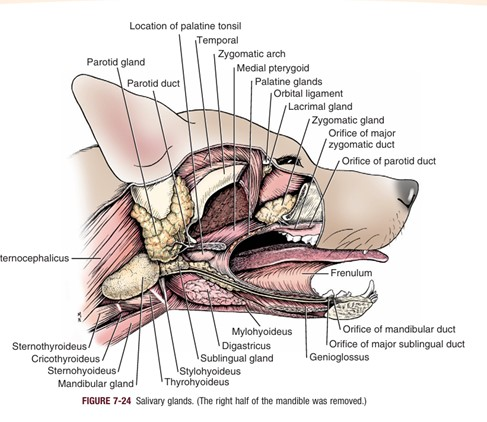
\includegraphics[width=0.99\textwidth]{../Figures/glls.jpg}
  \caption[Caption for figure in TOC.]{Caption for figure.}
  \label{fig:ggglyjdfg}
\end{figure}

\subsubsection{Glândula sublingual}

A glândula sublingual é composta por duas porções: a glândula sublingual monostomática e a glândula sublingual polistomática. Ambas estão localizadas em proximidade ao ângulo da mandíbula,numa posição ligeiramente lateral e rostral em relação à glândula mandibular, partilhando \cite{Han2016} com esta a mesma cápsula fibrosa/fáscia. (\cite{evans_millers_2012}) \cite{Brown2016} Quando comparadas com os restantes pares de glândulas salivares maiores, constituem o par mais pequeno. (\cite{evans_millers_2012})


A glândula monostomática é responsável por uma secreção que é conduzida por um único ducto excretor, o ducto sublingual maior, o qual termina na carúncula sublingual, adjacente à porção rostral do frénulo da língua. (\cite{evans_millers_2012}, Singh2017) Anatomicamente, a glândula consiste num agregado de duas ou mais massas lobulares, cuja extremidade se estende rostromedialmente. Localiza-se entre a borda caudomedial do músculo masséter (lateralmente) e o músculo digástrico (medialmente). Ao atingir a superfície lateral do músculo estiloglosso, a glândula curva-se rostralmente, posicionando-se medialmente ao corpo da mandíbula. \cite{evans_millers_2012}


A vascularização arterial da glândula monostomática é assegurada por ramos glandulares da artéria facial, enquanto a drenagem venosa ocorre pelas veias satélites associadas. \cite{evans_millers_2012}


A glândula polistomática corresponde à porção da glândula sublingual cuja secreção é drenada diretamente para a cavidade oral através de múltiplos ductos excretores independentes, os quais se abrem individualmente na mucosa do soalho da boca, sem confluírem num ducto comum nem formarem uma prega sublingual. (Singh2017)\cite{lobprise_oral_2019} Esta glândula é composta por seis  a 12 lóbulos de tecido glandular isolado, localizados rostralmente ao nervo lingual, encontrando-se anatomicamente separada da porção monostomática. \cite{evans_millers_2012}


A irrigação arterial da glândula polistomática é assegurada pela artéria sublingual, ramo da artéria lingual, e a sua drenagem pelas veias satélites associadas. \cite{evans_millers_2012}


A inervação parassimpática de ambas as porções da glândula sublingual é semelhante \cite{Han2016} à da glândula mandibular. A principal diferença reside na localização da sinapse parassimpática, que, no caso das glândulas sublinguais, ocorre no gânglio sublingual, localizado na proximidade da zona onde o nervo lingual cruza com o ducto sublingual maior. \cite{evans_millers_2012}

\subsubsection{Glândula zigomática}

A glândula zigomática, anteriormente designada como glândula orbital, é exclusiva de carnívoros domésticos, nomeadamente cães e gatos. Está localizada ventralmente à extremidade rostral do arco zigomático, tendo por isso um acesso relativamente difícil.\cite{lobprise_oral_2019,evans_millers_2012} 
Anatomicamente, apresenta um formato variável entre piramidal e globular. 

Esta glândula secreta saliva para a cavidade oral por intermédio de um ducto principal e até quatro ductos acessórios menores, os quais abrem na porção caudal do vestíbulo bucal. \cite{lobprise_oral_2019}
A vascularização arterial da glândula zigomática é assegurada principalmente por um ramo da artéria infraorbitária, enquanto a sua drenagem venosa é realizada por uma veia aferente que se junta à veia facial profunda. \cite{evans_millers_2012}

A inervação parassimpática secretomotora tem origem em neurónios pré- ganglionares localizados no nervo glossofaríngeo que seguem através do nervo timpânico pelo plexo timpânico na cavidade timpânica, que deixa a cavidade pelo nervo petroso menor e realiza sinapse no gânglio ótico. Os neurónios pós-ganglionares seguem então via nervo auriculotemporal, ramo do nervo mandibular, até atingirem a glândula zigomática. \cite{evans_millers_2012}

\subsection{Função da saliva}

A principal função das glândulas salivares é a produção de saliva, essencial para a proteção, lubrificação e manutenção da homeostase da cavidade oral durante a ingestão de alimentos. Esta forma uma camada seromucosa que protege o epitélio da cavidade oral contra agentes irritantes, dificultando a adesão de agentes patogénicos e impedindo a ação proteolítica de microrganismos.  


No processo de perceção gustativa, a natureza hipotónica facilita a dissolução de partículas alimentares, promovendo o contacto eficaz com os recetores gustativos. (textbook) Contém ainda gustina, proteína fundamental ao desenvolvimento e manutenção dos botões gustativos. (textbook) A mucina contribui para a viscosidade e lubrificação, (textbook) facilitando a mastigação e deglutição. (vários) 
A saliva desempenha também uma ação de limpeza mecânica da cavidade oral, removendo detritos alimentares, células descamadas e bactérias não aderentes. Além disso, limita a utilização de substratos, como os hidratos de carbono, por microrganismos orais , reduzindo assim o seu papel fermentativo.


O seu conteúdo em bicarbonato e fosfato confere-lhe propriedades tampão, regulando o pH da cavidade oral.
Do ponto de vista imunitário, contém substâncias com propriedades antimicrobianas, como lisozima, lactoferrina e imunoglobulina A, que atuam na defesa inata da cavidade oral contra agentes infeciosos. \cite{Mescher2018}


Em Medicina Veterinária, a saliva de cão tem sido explorada sobretudo como método não invasivo na deteção de biomarcadores, como o cortisol, cuja concentração varia consoante o porte do animal (cães de maior porte tendem a apresentar menor concentração de cortisol na saliva), estado reprodutivo (esterilizado ou intacto) e ritmo circadiano.\cite{damian_serial_2018,Pasha2018} Recentemente, tem também sido alvo de investigação na avaliação de parâmetros inflamatórios, como a proteína C reativa e adiponectina, com vista ao monitoramento da inflamação sistémica de forma menos invasiva.\cite{Pasha2018} 

\subsubsection{Composição e pH da saliva}

\subsubsection{Composição da saliva}

A saliva é um fluido seromucoso composto por uma complexa mistura de substâncias orgânicas e inorgânicas, incluindo eletrólitos, proteínas, vitaminas, hormonas, enzimas e moléculas com ação antimicrobiana. \cite{lobprise_oral_2019}

A composição da saliva varia muito entre espécies e tipo de glândulas \cite{Das_Textbook}

Nos cães, a saliva apresenta níveis elevados de cálcio e potássio, essenciais à remineralização dentária. (valor) Em comparação com humanos, verifica-se maior concentração de certos minerais (cálcio, sódio e potássio), mas menor concentração de fosfato. (valor)

Do ponto de vista enzimático, a atividade da amílase salivar é muito reduzida em cães, (amílase, alfa-amílase) tornando a sua contribuição para a digestão de hidratos de carbono praticamente irrelevante. (Cunningham, composição) A lípase lingual, presente em animais jovens, desaparece com a maturação. (Cunningham) Além disso, a salivava canina contém esterases não específicas, fosfatase ácida e pseudocolinesterase. (Cunningham) A saliva canina contém também cobalofilina, uma glicoproteína que se liga à cobalamina (ou vitamina B12) e a protege da secreção gástrica presente no estômago. (Textbook) 

\subsubsection{Ph da saliva}

A saliva dos canídeos possui um pH mais elevado em comparação com a humana (8,5 vs. 6,5-7,5), o que lhes confere uma maior capacidade tampão e protege o esmalte contra a desmineralização. (outro) Este pH mais alcalino contribui para uma menor incidência de cáries, mas favorece a formação de cálculos dentários, predispondo à gengivite e doença periodontal devido à deposição de sais de cálcio. (valor,outro)    

\subsubsection{Controlo nervoso da secreção salivar}

O fluxo salivar é contínuo e, embora a sua taxa de secreção seja influenciada por inúmeros fatores, é principalmente regulada pelo sistema nervoso autónomo, com predominância da componente parassimpática. (\cite{Poirier2018} histologic \cite{Bae2024},Singh2017) Embora ambos os ramos – simpático e parassimpático – possam estimular a secreção salivar de forma sinérgica, a ação parassimpática é predominante na regulação basal. \cite{lobprise_oral_2019},textbookphys) 
Os centros reguladores encontram-se localizados nos núcleos salivatórios da medula oblongata. \cite{lobprise_oral_2019}


As fibras parassimpáticas responsáveis pela estimulação das glândulas salivares originam-se em dois núcleos salivatórios localizados na medula oblonga . (\cite{Poirier2018} histologic \cite{Bae2024}) Estímulos aferentes de natureza visual, gustativa ou olfativa são transmitidos até esses núcleos, desencadeando impulsos eferentes que percorrem inicialmente os nervos facial (VII par craniano) e glossofaríngeo (IX par craniano). (Singh2017)Posteriormente, estas fibras são conduzidas até às glândulas alvo através de diferentes ramos do nervo trigémeo (V par craniano). (Singh2017) A estimulação parassimpática resulta na secreção de saliva em grande volume, geralmente associada a vasodilatação local. (Singh2017)


As fibras simpáticas têm origem nos segmentos torácicos caudal da medula óssea na túnica adventícia das artérias (\cite{Poirier2018} histologic \cite{Bae2024}) e terminam no gânglio cervical superior após passarem a cadeia cervical simpática. Estimulação é seguida por vasoconstrição, que reduz a taxa de produção e altera a sua composição. (Singh2017) (\cite{Poirier2018} histologic \cite{Bae2024}) O sistema simpático pode, por vezes, aumentar também a taxa de secreção, ao contrair as células mioepiteliais que, por sua vez, constringem o lúmen dos ácinos e dos ductos, aumentando a pressão nos ácinos e ductos. \cite{lobprise_oral_2019}


Contrariamente ao que se verifica noutras glândulas do sistema digestivo, a atividade secretora das glândulas salivares é exclusivamente controlada por mecanismos neurais, não estando sob regulação endócrina (Cunningham) Diversos fármacos podem influenciar a secreção salivar ao mimetizar os efeitos do sistema nervoso autónomo ou, indiretamente, ao modificar a perfusão sanguínea das glândulas salivares. \cite{Cattai2016} EQUIVALE(Acute postoperative sialadenosis) Estados emocionais como ansiedade, medo ou stresse, bem como a desidratação, têm um efeito inibitório sobre a produção salivar, podendo mesmo suprimi-la completamente em situações de maior gravidade. (\cite{Poirier2018} histologic \cite{Bae2024},Singh2017) 


\subsection{Sialoadenose em cães}

\subsubsection{Definição}

A sialoadenose é uma doença rara caracterizada por um aumento bilateral e indolor do parênquima das glândulas salivares, sem envolvimento inflamatório ou neoplásico. A glândula mais comumente afetada é a mandibular, embora a condição possa afetar outras glândulas salivares. ARTIGOSSS

\subsubsection{Fisiopatologia}

Na medicina humana, a sialoadenose é uma doença que representa cerca de 6\% de todos os diagnósticos de doenças das glândulas salivares. \cite{boydell_sialadenosis_2000} Nestes, aproximadamente metade dos casos relatados estão associados a disfunções de origem endócrina, metabólica, neurogénica ou nutricional, (\cite{Trinka2023}) sendo frequentemente observada em indivíduos com bulimia, anorexia nervosa, malnutrição, doença hepática, diabetes mellitus e neoplasia. \cite{Alcoverro2014} Face à diversidade de causas associadas em humanos, a fisiopatologia subjacente permanece pouco compreendida. \cite{Ide2011}


 A hipótese mais amplamente aceite em medicina humana foi proposta por Donath e Seifert, com base em investigações histológicas e ultraestruturais realizadas na década de 1970. Estes autores sugeriram que um distúrbio hormonal ou metabólico poderia desencadear uma neuropatia autonómica periférica. \cite{Davis2021} Tal disfunção comprometeria a estimulação das células mioepitelias e, adicionalmente, interferiria na atividade secretora exocitótica, conduzindo à acumulação de secreções nas células acinares e, consequentemente, ao aumento generalizado das glândulas salivares. \cite{Ihrler2010} Foram ainda observadas alterações estruturais características, como o aumento do volume das células acinares com acúmulo de grânulos secretores, bem como alterações degenerativas nas células mioepiteliais e nos nervos simpáticos pós-ganglionares, quando comparadas com indivíduos saudáveis. (\cite{Davis2021}, patogénese) A contração das células mioepiteliais depende do sistema nervoso autónomo, o que sustenta a hipótese de perda de estimulação em contexto de neuropatia autonómica periférica. \cite{Ihrler2010}


Pelo contrário, no caso dos cães, investigações clínicas e laboratoriais exaustivas nos casos presentes não revelaram qualquer doença primária de origem metabólica, gastrointestinal ou estrutural nas glândulas salivares. A ausência de alterações histológicas, aliada aos achados eletroencefalográficos e à resposta favorável ao tratamento com fenobarbital, suporta a hipótese de uma origem neurogénica, possivelmente associada a epilepsia límbica (EL) ou algum tipo de disfunção do sistema nervoso periférico. FALTA BIBLIO
Em suma, a disfunção da inervação do sistema nervoso autonómico poderá representar um mecanismo comum tanto em humanos como em animais. \cite{Alcoverro2014}


\subsubsection{Etiologia e hipótese neurológica: Epilepsia límbica}

\subsubsection{Epilepsia}

Epilepsia é a doença neurológica mais comum em cães, sendo caracterizada por uma predisposição crónica para a ocorrência de crises epiléticas recorrentes. (fvets-1-14) Esta condição engloba um conjunto heterogéneo de distúrbios neurológicos, apresentando manifestações clínicas diversas, variação na idade de aparecimento e múltiplas etiologias subjacentes. (\cite{loscher_dogs_2022}) 
A verdadeira prevalência de epilepsia em cães é desconhecida, mas estima-se que afete entre 0.6-0.75\% da população canina geral, valor comparável à prevalência observada em humanos. (\cite{von_ruden_role_2023},\cite{Packer2015},\cite{loscher_dogs_2022})


Com base na etiologia, a epilepsia em cães pode ser classificada em duas categorias:
 \begin{enumerate}
    \item Epilepsia estrutural: caracterizada por crises epiléticas associadas a lesões cerebrais identificáveis, como doenças vasculares, inflamatórias/infeciosas, traumáticas, adquiridas, neoplásicas e degenerativas);
    \item  Epilepsia idiopática: na ausência de lesões estruturais ou causas identificáveis, em que se presume o envolvimento de uma componente genética ou hereditária. (\cite{Packer2015})
\end{enumerate}


Num estudo retrospetivo envolvendo 900 cães submetidos a ressonância magnética após episódios convulsivos, foram identificadas lesões estruturais em 45,1\% dos casos, enquanto 54,9\% dos cães não apresentavam quaisquer alterações detetáveis. \cite{loscher_dogs_2022}
A característica clínica mais marcante da epilepsia, e o principal alvo terapêutico, é a crise epilética. Com base na manifestação das crises, as epilepsias podem ser classificadas em focais, generalizadas, focais e generalizadas (combinadas) e de origem desconhecida. 


As crises são consideradas generalizadas quando envolvem ambos os hemisférios cerebrais e focais quando a ocorrência de atividade elétrica anormal se encontra confinada a uma área específica do cérebro, resultando assim, em sinais clínicos divergentes, que vão depender diretamente da função da área cerebral envolvida. Estas podem, no entanto, desenvolverem e tornarem-se generalizadas. As crises focais foram relatadas em cães com epilepsia idiopática e estrutural e podem ocorrer com ou na ausência de consciência. (\cite{Packer2015})


\subsubsection{Epilepsia límbica}

Uma das hipóteses patofisiológicas mais discutidas na literatura propõe que a sialoadenose responsiva a fenobarbital (SRF) em cães represente uma manifestação de EL. (\cite{Kalayanakoul2019},\cite{gibbon_phenobarbital-responsive_german_2004},\cite{gibbon_phenobarbital-responsive_german_2004}) Esta forma de epilepsia caracteriza-se por convulsões epiléticas que se originam e/ou envolvem este sistema, (reid and staba, \cite{gibbon_phenobarbital-responsive_german_2004}) responsável por funções relacionadas com emoção, memória, motivação, comportamento e regulação de várias funções autonómicas. (\cite{gibbon_phenobarbital-responsive_german_2004},\cite{Bandusena2022})


Este envolvimento autonómico é particularmente relevante na interpretação dos sinais clínicos observados. Em Medicina Humana, foram descritas convulsões autonómicas com manifestações gastrointestinais (como ânsia de vómito, sialorreia, náusea, vómito, desconforto abdominal, borborigmos e diarreia), alterações do ritmo cardíaco (bradicardia e taquicardia) e do tamanho pupilar (midríase e miose) entre outros. (JVIM-39,10.10) Embora em Medicina Veterinária este tipo de apresentação seja raramente reconhecido, a SRF poderá constituir uma das primeiras descrições clínicas de crises epiléticas com expressão autonómica. \cite{Diop2025}


Em cães, a EL é habitualmente classificada como um tipo de epilepsia focal, que pode manifestar-se com sinais primários ou complexos. No entanto, conforme descrito em Seizures In cats and dogs, a escassez de evidência clínica impede muitas vezes a categorização inequívoca destas crises como focais ou generalizadas. Reconhece-se ainda que crises com origem no sistema límbico podem propagar-se a áreas neocorticais e vice-versa. 


O diagnóstico destas crises permanece um desafio, uma vez que os sinais clínicos são frequentemente mal interpretados e atribuídos a outras doenças. \cite{Diop2025}
Uma das principais evidências que sustentam a hipótese de EL na SRF é a presença de alterações eletroencefalográficas. Em alguns cães afetados, os registos obtidos através deste método, considerado padrão de referência no diagnóstico de epilepsia, estes revelaram padrões de atividade compatíveis com convulsões de origem no sistema límbico. \cite{gibbon_phenobarbital-responsive_german_2004} Contudo, também foram descritos casos com eletroencefalografia (EEG) normal, \cite{gibbon_phenobarbital-responsive_german_2004} o que dificulta uma confirmação diagnóstica inequívoca, sobretudo quando existe resposta positiva ao tratamento com fenobarbital, mesmo na ausência de achados eletrofisiológicos sugestivos.
A resposta favorável à terapêutica antiepilética, nomeadamente com fenobarbital (\cite{Alcoverro2014},13casos,\cite{gibbon_phenobarbital-responsive_german_2004}) e brometo de potássio, \cite{Alcoverro2014} tem sido recorrente nos casos descritos, reforçando a hipótese de envolvimento central na origem dos sinais clínicos.


O tratamento da SRF baseia-se sobretudo na administração de fenobarbital, um barbitúrico de primeira geração, de ação prolongada, amplamente utilizado principalmente no controlo de epilepsia. (\cite{Papich2021},\cite{Scott2021}) Este fármaco atua a nível do Sistema Nervoso Central (SNC), (\cite{Papich2021}) potenciando a atividade do neurotransmissor inibitório ácido gama-aminobutírico (GABA), (\cite{Trinka2023},chapter) o que resulta numa diminuição da excitibilidade neuronal. Apesar dos efeitos clínicos benéficos observados, não é possível afirmar de forma inequívoca que a SRF corresponda a uma forma de epilepsia, sendo plausível que o efeito do fármaco se deva a mecanismos alternativos ou indiretos. \cite{gibbon_phenobarbital-responsive_german_2004} Embora não haja evidência de que o fenobarbital interfira diretamente na motilidade esofágica ou na produção de saliva, sabe-se que este inibe a motilidade do intestino delgado, o que poderá justificar a existência de efeitos locais, ainda não completamente compreendidos. \cite{gibbon_phenobarbital-responsive_german_2004}


Importa ainda referir que, cães submetidos a \cite{Swieton2022} com SRF, os sinais clínicos persistem, o que sugere que o aumento físico das glândulas salivares não constitui a causa primária do quadro clínico. (\cite{Kalayanakoul2019}) 
Em suma, a combinação do quadro clínico, achados eletroencefalográficas, a resposta positiva à terapêutica antiepilética e a ineficácia da abordagem cirúrgica sustentam a hipótese de que a SRF poderá representar uma manifestação de EL, (varias refs) ou algum tipo de disfunção autonómica periférica. (\cite{gibbon_phenobarbital-responsive_german_2004})


\subsubsection{Sinais clínicos} 

Na clínica, os cães com sialoadenose apresentam uma variedade de sintomas que, na maioria dos casos, é caracterizado por um aparecimento súbito de ânsia de vómito e engolir em seco, frequentemente acompanhados por um aumento bilateral das glândulas salivares, especialmente as glândulas mandibulares. \cite{bsava_2020_gastro} Outros sinais clínicos comuns incluem engasgo,  ptialismo/sialorreia, lip smacking, perda de peso, hiporrexia ou anorexia, vómito crónico e/ou regurgitação. (boydel) Em casos de envolvimento da glândula zigomática, podem observar-se ainda exoftalmia, quemose e protusão da terceira pálpebra. (\cite{Park2022}, 12 casos) 


O exame físico, na maioria das vezes, não revela alterações significativas, com exceção de um aumento bilateral das glândulas salivares, sem sinais de dor à palpação. No entanto, os cães afetados podem revelar hipersensibilidade à palpação cervical que, pode desencadear episódios de gulping e retching, apesar de ausência de dor evidente. (boydel)

\subsubsection{Aumento bilateral das glândulas salivares} 

As doenças das glândulas salivares são relativamente raras em Medicina Veterinária. Quando ocorre aumento bilateral destas glândulas, as principais causas diferenciais incluem sialocele, sialoadenose, sialoadenite, sialometaplasia, infeção ou neoplasia das glândulas salivares.


De modo a avaliar e comprovar o aumento presente nas glândulas salivares, podemos recorrer à palpação ou por imagem, usando ultrassonografia, tomografia computorizada e ressonância magnética.

\subsubsection{Ptialismo} 

Como referido anteriormente, a saliva é produzida por quatro glândulas salivares principais-parótida, mandibular, sublingual e zigomática-bem como por um conjunto de glândulas salivares menores que também contribuem para a sua excreção na cavidade oral. (textbook medi nt)
Ptialismo, também denominado sialorreia ou hipersalivação corresponde a um aumento na produção e secreção de saliva, regulado maioritariamente pelo Sistema Nervoso Autónomo (SNA). Este deve ser diferenciado de pseudoptialismo, que se refere à incapacidade de deglutir ou reter a saliva na cavidade oral, normalmente devido a um processo patológico, apesar de a produção de saliva ser normal.
 Na prática clínica a distinção entre ptialismo verdadeiro e pseudoptialismo pode ser difícil, existindo até sobreposição de ambos os sinais. Assim, esta diferenciação requer uma investigação clínica minuciosa e continuada. \cite{bsava_2020_gastro}


O ptialismo e o pseudoptialismo podem ter inúmeras possíveis causas possíveis, sejam fisiológicas (característico de certas raças como o são bernardo, cocker spaniel, boxer, mastiff, dogue de bordeus, entre outras) \cite{canine_gastro_2013} ou patológicas, onde a causa primária pode ter origem na cavidade oral, por trauma ou doença oral, \cite{canine_gastro_2013}nas glândulas salivares, no esófago ou no trato gastrointestinal. (\cite{Kook2013}) Além disso, o ptialismo pode resultar de doenças neurológicas (centrais ou periféricas), distúrbios metabólicos, infeções, doenças autoimunes, causas congénitas, alterações comportamentais ou ainda ser induzido por fármacos ou tóxicos. (\cite{Kook2013}) 


O ptialismo verdadeiro é frequentemente observado em associação com náusea ou vómito, sendo mediado por vias neurais e humorais(canine). Nesses casos, a causa subjacente é, na maioria das vezes, de origem gastrointestinal, neurológica ou sistémica. \cite{ettinger_textbook_2010}


•	A presença de regurgitação aliada a ptialismo sugere fortemente uma afeção esofágica, sendo indicado um exame específico ao esófago.
•	Quando o ptialismo ocorre em conjunto com disfagia, levanta-se a suspeita de patologia oral ou maxilofacial, devendo ser realizado um exame físico detalhado dessas regiões. \cite{ettinger_textbook_2010}


No caso específico da sialorreia, sinal clínico frequentemente observado em casos de sialoadenose em cães, a produção excessiva de saliva pode ser explicada e associada a um aumento da atividade parassimpática ou alterações na inervação simpática. (12 cases) 


Nos casos presentes, existe um aumento das glândulas salivares sem uma anomalia a nível estrutural ou funcional documentada a nível da orofaringe, sugerindo assim, que a sialorreia, comumente presente nestas doenças, se deve ou a um aumento na produção de saliva ou relutância em engolir ao invés de uma alteração que leve à inabilidade de engolir. (Hypersialosis)

\subsubsection{Ânsia de vómito, engasgo e vómito crónico}

Engasgo (gagging) e ânsia de vómito (retching) são manifestações frequentemente observadas em simultâneo. (textbook) 
Após estímulos mecânicos ou irritativos, é desencadeada uma combinação de elevações rápidas e breves do palato mole acompanhada pela contração dos músculos constritores da laringe, levando à expulsão de material indesejado. (Textbook) Este reflexo, conhecido como engasgo, é um mecanismo de defesa que previne a entrada de corpos estranhos na faringe, laringe ou traqueia. (Textbook)


A ânsia de vómito caracteriza-se por um esforço involuntário e ineficaz de vomitar, habitualmente associado à náusea. Nestes casos, ocorre uma inversão da direção de fluxo e um peristaltismo descoordenado que resulta no contacto de ar com a glote fechada, o que origina o som típico do esforço sem produção de vómito. \cite{Das_Textbook} Quando estas tentativas se repetem, podem culminar no vómito efetivo. \cite{Das_Textbook}


Vómito ou emese é definido como a expulsão ativa e forçada do conteúdo gastrointestinal, resultante da contração da musculatura gastrointestinal, torácica e abdominal. \cite{Das_Textbook}Considera-se crónico quando persiste por um período igual ou superior a três a quatro semanas. \cite{bsava_2020_gastro} É um sinal clínico comum na prática veterinária, (\cite{Dixit2022}) exigindo uma abordagem sistemática que envolva uma compreensão clara da fisiopatologia e uma tomada de decisão clínica lógica. (\cite{Elwood2010}) O vómito pode ter origem em doenças gástricas ou não gástricas, (\cite{McGrotty2010}) e representa um mecanismo de defesa do organismo para remover agentes tóxicos, fármacos ou agentes infeciosos introduzidos por via enteral ou parenteral. \cite{Das_Textbook}


O vómito é facilitado por uma sequência de eventos organizados que requerem a coordenação gastrointestinal, musculoesquelética e do sistema nervoso (Vin) de modo a reduzir o risco de acontecimentos adversos como pneumonia por aspiração. Este reflexo é controlado no tronco cerebral, por uma zona designada como o “centro do vómito”. (\cite{Elwood2010}) Este centro recebe um estímulo de quatro áreas principais, o trato gastrointestinal, região vestibular, zona de gatilho quimiorrecetor  e córtex cerebral. \cite{Das_Textbook} Vias eferentes responsáveis pelo controlo destes processos incluem nervos vagais e frénicos, nervos do sistema parassimpático que se destinam às glândulas salivares e nervos somáticos motores dos músculos abdominais. (\cite{Elwood2010}) O reflexo de vómito tem normalmente 3 fases visíveis, de sialorreia, ânsia de vómito e expulsão. (\cite{Elwood2010}) 


Não obstante, os 3 sinais podem-se apresentar individualmente ou em conjunto, dado que tanto o engasgo e ânsia de vómito não implicam a ativação do reflexo de vómito. Por conseguinte, no caso do aparecimento individual destes sintomas, a etiologia pode diferir um pouco das causas típicas de \cite{Elwood2010,Das_Textbook}.  Em casos de sialoadenose, foi referido em alguns casos a presença de um destes sinais clínicos não acompanhado de vómito. (artigos)


\subsubsection{Regurgitação}

Regurgitação define-se como a expulsão passiva de alimento ou líquidos a partir do esófago, \cite{bsava_2020_gastro,canine_gastro_2013} sendo crucial distingui-la de vómito, \cite{_canine_gastro_2013} uma vez que essa diferenciação orienta a formulação correta dos diagnósticos diferenciais e a seleção de exames complementares mais adequados. \cite{bsava_2020_gastro}
A função principal do esófago é o transporte de sólidos e líquidos da cavidade oral até ao estômago. \cite{canine_gastro_2013} Para que esse processo ocorra normalmente, é necessário o relaxamento coordenado do esfíncter esofágico cranial, a integridade das contrações peristálticas e o relaxamento adequado do esófago caudal. \cite{_canine_gastro_2013}


\subsubsection{Hiporrexia, anorexia e perda de peso}

Anorexia define-se como ausência ou perda total de apetite, enquanto hiporrexia, embora não seja um termo estritamente padronizado, refere-se à redução parcial do apetite, sem supressão completa do mesmo. \cite{Delaney2006}
A regulação do apetite é um processo complexo que envolve a integração de múltiplos estímulos internos e externos em diferentes áreas do sistema nervoso central. \cite{canine_gastro_2013}Entre os fatores externos, destacam-se os estímulos sensoriais (particularmente o olfato, significativamente mais desenvolvido em cães e gatos do que em humanos), os hábitos alimentares, a localização das refeições e a sua temperatura -sendo que, alimentos servidos abaixo da temperatura corporal, tendem a ser menos aceites. \cite{_canine_gastro_2013}
Há também fatores orexígenos produzidos no sistema nervoso central, como o neuropéptido Y, que tem um papel central de regulação de apetite no hipotálamo, e a sua atividade depende essencialmente dos níveis de insulina e leptina circulantes. \cite{canine_gastro_2013}


Perda de peso ocorre por definição, sempre que o gasto de energia e as perdas calóricas superam a ingestão de nutrientes. Os principais determinantes deste desequilíbrio são o nível de apetite e o estado metabólico do paciente, ambos regulados por uma rede complexa de mecanismos neurais e hormonais. \cite{_canine_gastro_2013}


No contexto da sialoadenose, a perda de peso é frequentemente uma consequência direta da hiporrexia ou anorexia, que está presente na maioria dos casos clínicos descritos. A diminuição do apetite pode também resultar do desconforto associado aos episódios recorrentes de retching, gagging, náusea e sialorreia, contribuindo cumulativamente para a deterioração do estado corporal do animal.

\subsubsection{Diagnósticos diferenciais}

Devido à grande variedade de sinais clínicos, é essencial considerar e excluir outras afeções com manifestações semelhantes \cite{Han2016}, a fim de providenciar o tratamento mais adequado. A tabela seguinte apresenta os principais diagnósticos diferenciais a considerar:

% \usepackage{tabularray}
\begin{table}
\centering
\caption{Distribuição da casuística pelas três principais áreas clínicas, por espécie (Fip), frequência absoluta (Fi) e frequência relativa (Fr(\%))}
\label{tab:t1}
\begin{tblr}{
  width = \linewidth,
  colspec = {Q[263]Q[190]Q[229]Q[256]},
  cells = {c},
  cell{5}{1} = {c=4}{0.938\linewidth},
  hlines,
  vlines,
  hline{1,6} = {-}{0.08em},
}
Neoplasia da glândula salivar  & Sialoadenite        & Sialocele                & Sialometaplasia necrozante   \\
Sialolitíase                   & Esofagite           & Corpo estranho esofágico & Hipoadrenocorticismo atípico \\
Doença Inflamatória Intestinal & Neoplasia abdominal & Pancreatite              & Trauma do aparelho hióide    \\
Hérnia do hiato                & Gastrite            & Espirocercose            & Megaesófago~                 \\
Miastenia gravis               &                     &                          &                              
\end{tblr}
\end{table}

É importante destacar que, quando o ptialismo ocorre em associação com náuseas ou vómito crónico, a etiologia mais provável é de origem gastrointestinal, neurológica ou sistémica. Nestes casos, é indispensável realizar uma investigação clínica detalhada, com recurso a exames complementares apropriados. \cite{ettinger_textbook_2010}
A presença de regurgitação levanta suspeitas de uma possível afeção esofágica, sendo indicado proceder a exames como radiografia torácica ou endoscopia para confirmação diagnóstica. \cite{ettinger_textbook_2010}
O diagnóstico diferencial deve ser conduzido de forma criteriosa, assegurando que condições mais comuns- como as listadas acima- sejam devidamente excluídas antes de se confirmar o diagnóstico de sialoadenose.   
Adicionalmente, quando o ptialismo é acompanhado de disfagia, deve ser conduzida uma investigação minuciosa da cavidade oral e das estruturas maxilofaciais, de modo a excluir lesões orais ou maxilofaciais locais. \cite{ettinger_textbook_2010} 

\subsubsection{Alterações esofágicas como diagnóstico diferencial}

Está bem estabelecido que o diagnóstico de SRF em cães exige a exclusão rigorosa de causas identificáveis de sialorreia e vómito crónico, incluindo doenças inflamatórias, infecciosas, neoplásicas, metabólicas, neurológicas e gastrointestinais, com especial destaque para as condições esofágicas. 


Em relação a alterações esofágicas, como esofagite, megaesófago ou espirocercose, foi denotado sinais clínicos semelhantes \cite{Han2016} aos observados em casos de SRF, nomeadamente vómito/regurgitação, sialorreia e aumento das glândulas salivares. O aumento das glândulas salivares e a sua relação com problemas esofágicos não está completamente elucidada, no entanto, o mecanismo proposto baseia-se na existência de um reflexo esofagossalivar, onde impulsos aferentes provenientes do nervo vago (ativados por distensão e obstrução mecânica do esófago) atuam diretamente sobre os núcleos salivatórios, resultando na intensificação da secreção salivar. Foi demonstrado aumentos até 15 vezes superiores ao valor basal em ovinos e até 9 vezes superiores em seres humanos com obstrução esofágica.


Nestes casos, o tratamento da doença esofágica é de privilegiar, com descrição de melhoria dos sinais clínicos após a realização do mesmo. A resposta ao fenobarbital nestes contextos não é consensual, tendo sido descritos tanto casos de melhoria clínica, (10.4102) como casos sem qualquer resposta à terapêutica~\cite{Walton-Clark2022,gibbon_phenobarbital-responsive_german_2004}.

\subsubsection{Principais sialopatias em cães}
\subsubsection{Sialocele}
\subsubsection{Definição e etiopatogenia}

A sialocele, também denominada de mucocele ou rânula é, historicamente, a doença  mais comum que afeta as glândulas salivares. (\cite{deLaPuerta2020},\cite{Cinti2021},\cite{Olimpo2023}) É definido como um extravasamento e acumulação de saliva no tecido subcutâneo ou da submucosa, seguido por uma reação tecidual, onde ficam revestidos por uma cápsula composta por tecido conjuntivo inflamatório ao invés de um tecido epitelial típico. (\cite{Zadeh2025},\cite{rfeu},\cite{Bae2024},\cite{sa_})


As sialoceles ocorrem com maior frequência em cães comparativamente a gatos e não apresentam predisposição em termos de raça ou idade. (\cite{Bae2024}) O conhecimento sobre a etiologia é escasso, no entanto, foram propostas causas como cirurgia oral recente, sialólitos, corpo estranho, trauma e neoplasia. Entre estas, o trauma é a causa citada \cite{Kumar2017} mais frequentemente. (\cite{deLaPuerta2020}, \cite{Olimpo2023}) Contudo, na maioria dos casos, a causa específica permanece desconhecida. ({\cite{Cinti2021}}) Foi também revelado que alguns animais com sialocele, apresentam condições como hipercortisolismo ou tratamentos de longa duração com glucocorticoides. (\cite{Bae2024}) 


As mucoceles salivares são classificadas como cervical, sublingual, faríngeo ou zigomático consoante a glândula salivar comprometida. A glândula sublingual e o respetivo ducto são os mais frequentemente envolvidos. (\cite{Poirier2018}, \cite{Cinti2021},\cite{sa_})

\subsubsection{Sinais clínicos}

A maioria dos cães são assintomáticos e apresentam-se na clínica com história de um aumento gradual de uma massa flutuante não dolorosa. (\cite{Poirier2018}) No entanto, a sintomatologia pode ser variada e depende diretamente de qual a glândula acometida. (\cite{deLaPuerta2020}, \cite{sa_}) Sinais clínicos associados à glândula zigomática normalmente estão associados a exoftalmia e acumulação de saliva periorbital, enquanto sialoceles associadas  ao ducto ou glândulas sublinguais e mandibular manifestam-se usualmente com acumulação de saliva faríngea, sublingual ou cervical. (\cite{sa_}) Podem demonstrar também sinais de dor , hiporrexia/anorexia, halitose e sialorreia.  Se infetado, pode levar a descarga purulenta, pirexia e letargia (\cite{sa_}, \cite{Swieton2022})

\subsubsection{Diagnóstico}

O diagnóstico é baseado na história médica do paciente, sinais clínicos, citologia e por vários tipos de diagnóstico de imagem como radiografia, ultrassonografia, sialografia contrastada, Tomografia Computorizada (TC) e/ou ressonância magnética (RM). (\cite{Bae2024}, \cite{sa_},\cite{Olimpo2023},\cite{deLaPuerta2020}) Usualmente é \cite{Kumar2017}ado por punção aspirativa por agulha fina (PAAF) da tumefação, obtendo-se um fluido com aparência mucosa ou viscosa com pouca celularidade que, corada com o ácido periódico de Schiff (PAS, do inglês Periodic Acid-Schiff) nos confirma o diagnóstico. (\cite{Poirier2018}) A sialografia comprova  a rutura do complexo ducto/glândula em 55\% dos casos. (\cite{Olimpo2023}) 

\subsubsection{Tratamento e prognóstico}

O tratamento de escolha para as sialoceles é cirúrgico e requer excisão completa do complexo glândula/ducto por abordagem ventral ou lateral para ser curativo e evitar recorrências. (\cite{Poirier2018}, \cite{Swieton2022}) Recorrências após cirurgia estão entre 5-14\% dos casos, tendo por isso um prognóstico favorável. (\cite{Poirier2018}) Recorrências ocorrem maioritariamente no primeiro ano após a cirurgia. (\cite{Swieton2022}) Há também a possibilidade de realizar radioterapia como forma de controlo ou em casos refratários de maneio cirúrgico. (\cite{Poirier2018})

Sialoadenite
\subsubsection{Definição e etiopatogenia}
A sialoadenite tem sido descrita como a doença mais comum das glândulas salivares em estudos mais recentes, com uma prevalência de $49,7\%$  ($89/179$ casos). (sialadenite+sialocele;lieske)

Sialoadenite e sialoadenose são doenças caracterizadas por um aumento das glândulas salivares (\cite{Enache2025}) Sialoadenite é uma doença inflamatória rara presente nas glândulas salivares, que pode ser causada por infeção local ou sistémica, trauma ou doença autoimune. (\cite{supurativa},\cite{11cases}, \cite{sialadenite}) É também possível que ocorra por consequência e secundariamente a náusea crónica, regurgitação ou vómito associados a uma causa gastrointestinal primária. (\cite{McGill2009}) No estudo com o maior número de animais citados \cite{Kumar2017} com sialadenite ($n=20$ casos) foi verificado que, tal como em pessoas, existe a possibilidade de uma correlação com outras doenças sistémicas, como doenças gastrointestinais, anorexia/hiporrexia ou até doença renal crónica, hipotiroidismo e diabetes mellitus. (\cite{11cases}, \cite{Enache2025}) Embora descritas estas possíveis causas, a fisiopatologia da doença mantém-se desconhecida. (\cite{sialadenite}) Em outros estudos  efetuados, alguns cães demonstraram resposta benéfica ao tratamento com fenobarbital, tendo sido proposto que a sialadenite   poderia estar, tal como a sialoadenose, associada a uma forma atípica de epilepsia límbica. (\cite{Martinez2018},\cite{Park2022}) 
\subsubsection{Sinais clínicos}
Os sinais clínicos predominantes são o aumento de tamanho individual ou bilateral das glândulas salivares, associado a sialorreia, tumefação, dor e/ou outros sinais clínicos de resposta inflamatória. (\cite{McGill2009}) Se a sialadenite ocorrer na glândula zigomática, pode levar a sinais clínicos característicos de doença retrobulbar, estrabismo, protrusão da glândula da terceira pálpebra, enoftalmia e diminuição ou ausência de retropulsão do olho. (\cite{11cases})
subsubsection{Diagnóstico}
O diagnóstico definitivo desta condição é idealmente realizado com base nos resultados da citologia e/ou histopatologia da glândula ou par de glândulas afetadas, com associação a culturas e testes de sensibilidade a antibióticos (TSA). (\cite{Enache2025}) O resultado da citologia/histopatologia   revela normalmente inflamação predominantemente neutrofílica. (\cite{Enache2025}) É, no entanto, essencial a associação dos indícios obtidos na história médica, no exame físico e com recurso a outros meios complementares de diagnóstico, como a ultrassonografia, RM e/ou TC  (\cite{Enache2025})

\subsubsection{Tratamento e prognóstico}

O tratamento consiste normalmente no uso de antibioterapia, baseada idealmente nos resultados da cultura e do TSA, com associação a anti-inflamatórios não esteroides (AINE’s) ou corticosteroides, analgesia e tratamento dirigido à doença sistémica associada. (\cite{Park2022}, \cite{Enache2025},\cite{sialadenite}) O fenobarbital tem sido reportado como tratamento único em cães que apresentem sialoadenite não responsivo ao uso de antibióticos e como tratamento adjuvante de cães com necrose de as glândulas salivares. (\cite{Park2022},\cite{Enache2025}) Foi referido também a possibilidade de a administração precoce com fenobarbital ser benéfico para a resolução de sinais clínicos em casos de sialoadenite zigomática. (\cite{Martinez2018})


A maioria dos casos identificados na literatura teve um prognóstico bom, com resolução dos sinais clínicos e sem evidência de recorrência. (\cite{sialadenite}) Importante denotar que existe pouca literatura e informação sobre esta condição, sendo por isso difícil assumir uma resposta confiável em relação ao prognóstico da mesma.   
No caso de existir mais que um par de glândulas afetadas e citados \cite{Kumar2017} com sialoadenite, apesar de uma possível resposta inicial positiva, há uma maior probabilidade de recorrência, havendo assim, a possibilidade de que o tratamento com fenobarbital e o prognóstico se torne pobre no caso de mais que uma glândula salivar se encontrar alterada. (\cite{Park2022})

  
Neoplasias das glândulas salivares
Definição e etiopatogenia


Neoplasias presentes nas glândulas salivares em cães e gatos é um acontecimento raro, tendo uma incidência de cerca de 0.17\% de todas as condições neoplásicas em cães sendo, no entanto, uma causa significativa de doença salivar. (\cite{Almeida2010}, withrow, \cite{Oshikata2006},\cite{Hammer2001},\cite{campos2019},\cite{Cray2020}, \cite{deLaPuerta2020}) A maioria das neoplasias das glândulas salivares são malignas e de origem epitelial, sendo o adenocarcinoma simples o tipo primário mais comum. (\cite{Almeida2010}, withrow, \cite{Oshikata2006},\cite{Hammer2001},\cite{campos2019},\cite{Cray2020}, \cite{deLaPuerta2020}) Outros tipos de carcinoma representam a segunda causa mais frequente. (withrow) Foi reportado também a presença de outros tipos de neoplasias que incluem fibrossarcoma, lipoma, oncocitoma, adenoma pleomórfico, mioepitelioma, osteossarcoma, mastocitoma e linfoma. (veterinary, withrow,\cite{Cray2020})


A glândula parótida é a mais afetada em cães, com uma tendência de predisposição superior  observada na raça Caniche . (veterinary, \cite{Oshikata2006}) Acomete geralmente animais geriátricos (média de 13.4 e 10.5 anos em gatos e cães respetivamente) e não demonstra predisposição sexual. (\cite{Cray2020}, \cite{deLaPuerta2020})


Em termos de metastização em cães, dois estudos com amostras significativas apresentaram incidências distintas, facto que pode ser justificado pelas diferenças no tipo de neoplasias avaliadas. O primeiro estudo, que incluiu vários tipos de neoplasias das glândulas salivares, relatou uma taxa de metastização para linfonodos locais de 17\% e 8\% para metastização à distância. Por outro lado, o segundo estudo, mais recente e com uma amostra maior (n=69 vs n=24 casos), focado exclusivamente em carcinomas das glândulas salivares, observou taxas superiores: 28.9\% para linfonodos regionais e 31.9\% para metastização à distância. (*Vete ,Outcomes)


Sinais clínicos


O motivo de consulta mais frequente foi a presença de uma massa. Outros sinais clínicos incluem halitose, disfagia, dor, perda de peso, anorexia, ptialismo, síndrome de horner e espirros. (\cite{Dobson2011}, withrow, *Vete) 


Diagnóstico


O diagnóstico e tratamento precoce são relatados como fatores que melhoram significativamente o tempo de sobrevivência em cães. (\cite{Dobson2011}) Com isso em mente, recomenda-se a realização de PAAF da massa, de forma a distinguir a presença ou ausência de um processo neoplásico, bem como determinar se é benigno ou maligno. (\cite{Dobson2011}, onco) No caso de resultado insatisfatório, a realização de biópsia incisional ou excisional, seguida por histopatologia deve ser considerada. (withrow) Dado o potencial metastático e agressividade local característico de carcinomas, assim como outros tumores malignos , deve-se complementar o planeamento cirúrgico com exames complementares que permitam o estadiamento, tal como a citologia dos linfonodos locais, TC e/ou radiografia torácica. (withrow, \cite{Dobson2011})
Tratamento e prognóstico
A remoção cirúrgica da glândula afetada (sialoadenectomia), é considerado o tratamento primário para o controlo local da doença, em ambos humanos e animais. (Vete, \cite{Dobson2011}, withrow) Como referido anteriormente, as glândulas mandibulares e sublinguais estão intimamente associadas uma à outra em termos de localização e partilham a mesma cápsula levando a que, quando uma destas está afetada, ambas são removidas. (Vete) 
No que diz respeito às complicações associadas a sialoadenectomia secundária a carcinoma de glândula salivar, as principais são formação de seroma e dano a nível do nervo facial, localizado em estreita proximidade à glândula parótida, levando a paresia eou paralisia da face. (Vete, Withrow, Vete)
O tempo médio de vida em cães e gatos com tumores de glândula salivar após a sialoadenectomia foi semelhante \cite{Han2016}, sendo de 550 e 516 dias respetivamente.  (\cite{Hammer2001},\cite{Dobson2011},VETE,Withrow) Outro estudo reporta que cães submetidos a tratamento cirúrgico para carcinoma salivar apresentaram um tempo médio de sobrevivência de 1.886 dias, com uma taxa de recorrência local de 42\% e um intervalo livre de doença de 191 dias. Metástases foram observadas em 31,9\% dos casos, com um intervalo livre de doença de 299 dias. A presença de metástases em linfonodos locais, identificada em 28,9\% dos cães, foi considerada um fator prognóstico negativo, estando associada a um intervalo livre de doença de apenas 98 dias (Vete)


Tratamento adjuvante com quimioterapia no período pós-cirúrgico demonstrou impacto reduzido e elevada variabilidade no tempo médio de sobrevida em animais com carcinoma das glândulas salivares. Portanto, são necessários estudos adicionais para elucidar a sua eficácia. (Vet,\cite{Hammer2001})

Sialometaplasia necrosante
Definição e etiopatogenia


Sialometaplasia necrosante é uma lesão benigna auto limitante das glândulas salivares, caracterizada histologicamente	por necrose isquémica lobular das glândulas sero mucinosas acompanhado de metaplasia escamosa dos ácinos e ductos. \cite{Mukaratirwa2015,reiter_bsava_2018} 


A sua ocorrência é rara e pode ocorrer tanto cães como gatos. A etiologia permanece desconhecida e tanto a história e apresentação clínica é semelhante \cite{Han2016} à sialoadenose. Por essa razão, especula-se a possibilidade de sialoadenose progredir para um quadro de sialometaplasia necrosante. \cite{reiter_bsava_2018} A condição acomete usualmente as glândulas mandibulares, assim como a sialoadenose, embora relatórios de caso descrevam a sua presença em outras glândulas, como a zigomática e parótida. (\cite{perez-ecija_granulomatous_2012},kim) Suspeita-se de uma patogénese neurogénica correlacionada a anomalias do nervo vago  e está associada a condições e afeções esofágicas como espirocercose (por Spirocerca lupi), corpo estranho esofágico, divertículo esofágico, esofagite, giardíase e sialoadenite. \cite{reiter_bsava_2018,schoroeder}, kim)


Sinais clínicos


A apresentação clínica mais comum de sialometaplasia necrosante em cães inclui náusea, disfagia, dor na região mandibular, ânsia de vómito, vómito crónico, regurgitação, ptialismo, estalar dos lábios (lip smacking), perda de peso, anorexia, prostração e engasgo. \cite{Mukaratirwa2015,reiter_bsava_2018} 


Diagnóstico


O diagnóstico definitivo de sialometaplasia necrosante requer biópsia incisional e avaliação histopatológica. Modalidades de imagiologia avançada, como RM e TC, devem ser consideradas, assim como a avaliação citológica da glândula afetada por PAAF. \cite{reiter_bsava_2018}


Deve ser considerada a realização de radiografia torácica e endoscopia esofágica, complementada com exame coprológico, para descartar etiologias como espirocercose e corpo estranho esofágico, comumente associadas a sialometaplasia necrosante. (spirocerca,BSAVA, \cite{schoroeder},kim) Embora a sialometaplasia necrosante apresente um comportamento benigno em pacientes humanos e cães, a ocorrência de metaplasia escamosa pode levar a erros de diagnóstico, sendo erroneamente confundida com carcinoma. Isso pode resultar em tratamentos inadequados, como cirurgia radical e quimioterapia. (kim,\cite{Mukaratirwa2015})


Tratamento e prognóstico


Em cães, a escassez de base de dados dificulta a obtenção de conclusões sobre o curso clínico típico, tratamento e prognóstico. \cite{bsava_2020_gastro,Mukaratirwa2015} A remoção cirúrgica da glândula afetada apresenta resultados variáveis, havendo grande probabilidade de recorrência. \cite{Mukaratirwa2015,bsava_2020_gastro} O tratamento médico inclui maneio de dor, AINE’s, glucocorticoides em dose anti-inflamatória, controlo de parasitas internos (\textit{Giardia spp.} e \textit{Spirocerca spp.}) e administração de fenobarbital. \cite{reiter_bsava_2018} O seu prognóstico é reservado. \cite{bsava_2020_gastro,Mukaratirwa2015,reiter_bsava_2018}



Sialolitíase
Definição e etiopatogenia


Sialolítiase é definida como a formação de cálculos na glândula salivar ou respetivo ducto e tem sido reportada infrequentemente em veterinária, apesar de totalizar 30\% das afeções a nível das glândulas salivares em humanos. (\cite{perez-ecija_granulomatous_2012},\cite{Han2016},\cite{Ryan2008}) Em cães, os sialólitos ocorrem normalmente unilateralmente no ducto salivar da glândula parótida, sendo compostos maioritariamente por minerais inorgânicos de carbonato de cálcio e fosfato de cálcio. (\cite{perez-ecija_granulomatous_2012}, \cite{Han2016}) A etiologia da condição permanece desconhecida, mas foi sugerida uma associação com fluxo salivar reduzido, secundário a sialoceles crónicas e transposição do ducto parotídeo. \cite{perez-ecija_granulomatous_2012,Han2016,Ryan2008} Complementarmente, ambas as condições podem favorecer o aumento do número de bactérias na glândula ou ducto salivar afetado, seja por retenção salivar ou pela entrada de bactérias secundária a conjuntivite bacteriana. (\cite{Han2016}) 
Em termos de incidência, a presença de sialólitos é mais comum em cães de meia-idade a idosos. (\cite{Han2016}) 


Concluindo, a sialolitíase canina aparenta ser uma doença adquirida, resultante de um processo crónico, como sialoceles e infeções bacterianas. (\cite{Han2016})


Sinais clínicos


A maioria dos casos de sialolitíase em cães apresentam aumento não doloroso da glândula ou ducto afetado. \cite{Han2016,perez-ecija_granulomatous_2012}Outros sinais como pirexia, dor, corrimento ocular mucopurulento e sialorreia também foram reportados. (\cite{Han2016})


Diagnóstico



Geralmente, a sialolitíase pode ser facilmente citada \cite{Kumar2017} por meio de radiografia, uma vez que a maioria dos sialólitos são radiopacos, devido à sua composição rica em cálcio. (\cite{Han2016}) No entanto, caso o resultado da radiografia não seja conclusivo, sialografia contrastada, ultrassonografia, RM e TC são alternativas viáveis para a obtenção de um diagnóstico definitivo. (\cite{Han2016}) Entre esses meios, a TC foi considerada a mais específica e detalhada, por permitir determinar com precisão a localização exata do sialólito. \cite{Han2016,perez-ecija_granulomatous_2012}


Tratamento e prognóstico


O tratamento de sialolitíase consiste na remoção cirúrgica do sialólito e é geralmente eficaz, apresentando baixa taxa de recorrência e poucas complicações graves. \cite{Han2016,Ryan2008,perez-ecija_granulomatous_2012} Se os sialólitos estiverem localizados no ducto salivar na ausência de sialocele, podem ser removidos por meio de incisão no ducto, utilizando uma abordagem percutânea ou transoral. (\cite{Han2016}) 
No caso de se apresentarem na glândula salivar e estarem associados a sialocele, recomenda-se a remoção da glândula e ducto afetado de modo a prevenir a recorrência dos mesmos. (\cite{Han2016})
Tendo por base esta informação, o prognóstico é bom.


Exames Complementares e Diagnóstico de Sialoadenose de origem neurológica

Quando um clínico é abordado por um cão com glândulas salivares aumentadas e vómito crónico, é fundamental realizar uma avaliação diagnóstica criteriosa. (4 casos, case report) 
A sialoadenose é considerada uma condição de diagnóstico por exclusão, dado que não existem alterações específicas nos exames complementares que permitam confirmá-la e, ainda não foi estabelecido um teste de referência (“gold standard”) para a sua identificação. (rotweiller,4 casos, case report, VMS) 


O diagnóstico baseia-se, portanto, numa abordagem sistemática de exclusão, começando pela necessidade de descartar doenças primárias ou secundárias do trato gastrointestinal, que frequentemente se manifestam com sinais semelhantes, como vómito crónico e sialorreia/ptialismo. (4 casos, case report, VMS)


As principais condições sistémicas que causam vómito crónico- como doença renal crónica, doenças hepatobiliares, diabetes mellitus e hipoadrenocorticismo- podem ser identificadas através da avaliação do hemograma completo (CBC), perfil bioquímico sérico e análise urinária. (\cite{Leib2010}) Nos casos em que estas doenças são excluídas, a investigação deve centrar-se nas causas gastrointestinais mais frequentes, tais como: gastrite crónica, doença inflamatória intestinal (IBD), corpo estranho gástrico, hipertrofia pilórica, adenocarcinoma gástrico, linfoma gastrointestinal e obstruções parciais do intestino delgado. (\cite{Leib2010})


Após a exclusão das doenças sistémicas gastrointestinais, devem também ser consideradas e descartadas outras sialopatias mais comuns, como neoplasias, sialoadenite, sialoceles, sialolitíase e sialometaplasia necrosante, conforme previamente descritas. (4 casos, case report) 


Importa destacar que, além da exclusão criteriosa de outras doenças, a resposta clínica rápida e marcante ao tratamento experimental com antiepiléticos, como o fenobarbital, é um indicador fortemente sugestivo de sialoadenose. (4 casos, mais) Nestes casos, a melhoria evidente dos sinais clínicos apoia o diagnóstico presuntivo da condição, sobretudo quando os restantes diagnósticos diferenciais já foram devidamente afastados.


Para este processo, é essencial recorrer aos seguintes exames complementares: hemograma, perfil bioquímico sérico, urinálise, radiografia torácica, ecografia abdominal e teste de estimulação da hormona adrenocorticotrófica (teste estimulação de ACTH). Estes exames são indispensáveis para a exclusão das principais causas sistémicas associadas ao vómito crónico, e integram o algoritmo de diagnóstico de forma empírica, dado que, até ao momento, não existe um protocolo universalmente estabelecido. (fvets-10)


Hemograma + Perfil bioquímico sérico (Painel analítico geral??)


A realização de um painel analítico geral é um passo essencial no processo de diagnóstico por exclusão da sialoadenose, permitindo afastar uma ampla gama de condições sistémicas com sintomatologia semelhante, como vómito crónico e ptialismo. Entre os parâmetros avaliados, destacam-se aqueles relacionados com a função renal e hepática, uma vez que disfunções nestes órgãos estão frequentemente associadas a quadros gastrointestinais persistentes.

Avaliação da função renal

A análise da concentração de ureia tem como objetivo identificar potenciais disfunções renais ou hepáticas, enquanto a creatinina sérica é utilizada para avaliar a taxa de filtração glomerular, sendo um marcador mais específico da função renal. (rottweiler) 


Contudo, importa salientar que a creatinina apresenta sensibilidade limitada, já que os seus valores séricos permanecem dentro do intervalo de referência até que cerca de 75\% dos nefrónios já estejam comprometidos. \cite{Kovarikova2015}


Nessa perspetiva, torna-se revelante considerar marcadores alternativos como a dimetilarginina simétrica (SDMA), um biomarcador renal que se eleva precocemente em comparação com a creatinina, à medida que a taxa de filtração glomerular diminui. \cite{Gori2020} A SDMA apresenta ainda a vantagem de não ser influenciada pela massa muscular, ao contrário da creatinina. \cite{sdma}


Avaliação da função hepática


Como forma de avaliar a função hepática, o perfil bioquímico sérico inclui a análise de enzimas como a Aspartato aminotransferase (AST), alanina aminotransferase (ALT), fosfatase alcalina (ALP), $\gamma$-glutamil transferase (GGT). 


As enzimas ALT e AST são indicadores de lesão hepatocelular. A ALT é mais específica, pois está presente maioritariamente no citosol dos hepatócitos, enquanto a AST se encontra também presente nos miócitos. Quando ambas se encontram aumentas proporcionalmente, sugere-se lesão hepática; no caso de a AST estiver aumentada de forma desproporcional e associada a elevação da creatina quinase, deve-se considerar lesão muscular.


As enzimas ALP e GGT são consideradas marcadores de colestase, refletindo obstrução ou alteração do fluxo biliar intra ou extra-hepático. Ambas estão presentes na membrana canalicular dos hepatócitos e são fundamentais na avaliação de doenças hepatobiliares. A ALP possui enzimas de origem hepática, óssea e induzida por corticosteroides, dificultando por vezes a sua interpretação. A GGT, embora menos sensível que a ALP, é mais específica para doenças hepatobiliares. A avaliação combinada de ALP e GGT aumenta significativamente a especificidade para doenças hepáticas, atingindo mais de 90\%, comparativamente a 51\% com ALP isolada e 80\% com GGT isolada. 

COLOCAR ARTIGOSSS

Urinálise


A urinálise é um exame de rastreio fundamental, frequentemente subutilizado, que requer equipamento mínimo \cite{Ristic2011},\cite{Kumar2017} e fornece informações valiosas sobre a ocorrência e extensão de doenças do trato urinário como sobre sistémicas. \cite{Ristic2011},\cite{Yadav2020},\cite{Reine2005} Informações complementares podem ser obtidas através da submissão de amostras a um laboratório externo, seja para cultura bacteriana e teste de sensibilidade a antimicrobianos, seja para análises adicionais, como a determinação do rácio proteína/creatinina urinária. \cite{Ristic2011} 


De forma geral, a urinálise básica inclui testes com tiras reagentes (dipstick), o exame do sedimento urinário e determinação da densidade urinária específica. \cite{Ristic2011} 


Este exame permite identificar alterações compatíveis com doenças metabólicas, como diabetes mellitus, hepatopatias ou hemólise, através da deteção de glucose, corpos cetónicos, bilirrubina ou hemoglobina na urina, respetivamente. \cite{Parrah2013} 
Quando correlacionados com os resultados do perfil bioquímico, o exame físico e o historial clínico, os dados obtidos pela urinálise contribuem significativamente para a inclusão ou exclusão de diagnósticos diferenciais relevantes, como a doença renal crónica e a diabetes mellitus. \cite{Reine2005} Estas condições são causas frequentes de vómito crónico e devem sempre ser consideradas em casos suspeitos de sialoadenose.


Mensuração de Lípase pancreática canina

Lipase pancreática canina é considerada um dos biomarcadores mais sensíveis e específicos para o diagnóstico de pancreatite. \cite{Kim2024} Em condições fisiológicas, cerca de 99\% da lípase pancreática é libertada pelos polos apicais das células acinares pancreáticas, contribuindo para digestão de gorduras na dieta. \cite{Lim2022} O restante 1\% difunde-se pela membrana basolateral das células acinares, atingindo assim a circulação sistémica.\cite{Lim2022}


Durante processos inflamatórios pancreáticos, como a pancreatite, a secreção apical encontra-se comprometida. Como alternativa, há uma libertação aumentada de lipase para o espaço vascular através da via basolateral. \cite{Lim2022} Este mecanismo explica os níveis séricos aumentados de lípase em cães com inflamação pancreática.
A dosagem da lípase pancreática está incluída no perfil bioquímico sérico e assume particular importância no contexto de diagnóstico de exclusão de sialoadenose, dado que a pancreatite é uma das causas mais comuns de vómito crónico em cães. (Rottweiler) 


Contudo, é essencial salientar que o diagnóstico definitivo de pancreatite não deve basear-se exclusivamente nos níveis de lipase pancreática. A interpretação deste biomarcador deve ser realizada em conjunto com o historial clínico do animal, sinais clínicos compatíveis e achados ecográficos sugestivos de inflamação pancreática (\cite{Cridge2021},\cite{Kim2024}, \cite{Lim2022}).


Embora a Biópsia pancreática seja considerada o gold standard para o diagnóstico de pancreatite, é raramente usada dado o seu carácter invasivo, custo elevado e risco de não amostragem da lesão pancreática local. \cite{Cridge2021},\cite{Kim2024},\cite{Lim2022}, \cite{Liu2025}


Teste de estimulação da hormona adrenocorticotrófica (ACTH)


O teste de estimulação de ACTH é amplamente considerado o teste mais apropriado para a confirmação de hipoadrenocorticismo canino, apresentando elevada sensitividade e especificidade. \cite{Guzman-Ramos2022},\cite{Wakayama2017},\cite{Botsford2018},\cite{Spence2018},\cite{Mooney2023}


O hipoadrenocorticismo é uma condição endócrina relativamente rara, resultante da produção insuficiente de mineralocorticoides e/ou glucocorticoides pelas glândulas adrenais. (\cite{Guzman-Ramos2022},\cite{Wakayama2017},\cite{Mooney2023}) A condição pode ser classificada como primária, quando associada a falência adrenal, ou secundária, quando relacionada com disfunção hipofisária e consequente redução da secreção de ACTH. \cite{Botsford2018},\cite{Mooney2023}


Na maioria dos casos de hipoadrenocorticismo, a etiologia está associada a um processo imunomediado, que provoca destruição e subsequentemente fibrose do córtex adrenal. \cite{Wakayama2017},\cite{Spence2018},\cite{Mooney2023} 


Clinicamente, os animais afetados apresentam sinais pouco específicos, sendo os mais comuns: letargia acompanhada de uma variedade de sinais gastrointestinais, incluindo anorexia, regurgitação, vómitos, diarreia e perda de peso. \cite{Guzman-Ramos2022} Devido à sobreposição clínica com outras causas de vómito crónico, o hipoadrenocorticismo deve ser sempre considerado no contexto de diagnóstico de exclusão de sialoadenose.


O protocolo do teste de estimulação de ACTH envolve a colheita de uma amostra basal de sangue, seguida da administração de 5 µg/kg de ACTH sintético, por via intravenosa (preferencialmente) ou intramuscular.\cite{Spence2018}, \cite{Mooney2023} A segunda amostra é colhida 30 a 90 minutos após a administração da hormona. \cite{Spence2018}
Num cão saudável, os níveis de cortisol pós-ACTH deverão situar-se acima dos 250 nmol/L, refletindo uma resposta adrenal adequada. \cite{Mooney2023} Pelo contrário, cães com hipoadrenocorticismo apresentam concentrações persistentemente baixas, frequentemente próximas do limite de deteção do ensaio (~25 nmol/L). \cite{Mooney2023} Um valor inferior a 55 nmol/L após a estimulação é considerado consistente com o diagnóstico \cite{Wakayama2017}, \cite{Mooney2023}, \cite{Guzman-Ramos2022}.

Patologia clínica


No estudo com o maior número de pacientes diagnosticados com sialoadenose, que inclui apenas 12 casos, a amostra revela-se demasiado limitada para se poderem estabelecer conclusões sólidas acerca das alterações mais frequentemente observadas no painel analítico geral. Nesse estudo, refere-se apenas que nenhum dos animais apresentou anomalias significativas nesses parâmetros. \cite{boydell_sialadenosis_2000} No entanto, não são apresentados dados numéricos, tabelas ou descrições detalhadas que corroborem esta afirmação, nem é esclarecida a eventual presença de alterações mínimas.
No entanto, alterações como leucocitose, azotemia (possivelmente pré -renal) e hipocalemia têm sido descritas em diversos relatórios de casos. (maltes,2casos, case report,fenobarbital)


Anomalias eletrolíticas


Os níveis de potássio encontram-se consistentemente abaixo do limite inferior de referência em alguns casos, muito provavelmente devido aos episódios de vómito crónico observados em pacientes com sialoadenose. (4 casos) Adicionalmente, é referida a possibilidade de esta alteração eletrolítica estar relacionada com a elevada concentração de potássio presente na saliva, em comparação aos seus níveis séricos. Em cães, a concentração de potássio na saliva é aproximadamente 3-7 vezes superior à concentração no soro. (gillor2010, case report)


Endoscopia 


De modo a excluir outras patologias potencialmente responsáveis por vómito crónico, como esofagite, hérnia do hiato, corpos estranhos esofágicos ou gástricos, doença inflamatória intestinal, gastrite e massas abdominais, é frequentemente realizada endoscopia digestiva alta, procedimento amplamente utilizado na investigação de sinais gastrointestinais como ânsia de vómito, vómito, regurgitação ou diarreia (Maltês) \cite{mccarthy_veterinary_2021}.


Nos casos em que se suspeita de doença esofágica, manifestações como regurgitação, sialorreia, anorexia e perda de peso— sinais frequentemente sobrepostos aos observados na sialoadenose — podem justificar a realização de esofagoscopia, a qual permite não só a remoção de corpos estranhos, como também a avaliação direta da mucosa esofágica, identificando alterações como esofagite, divertículos ou sinais compatíveis com hérnia do hiato. \cite{Sum2009} Adicionalmente, permite a colheita de amostras para fim de avaliação histopatológica, citológica e microbiológica. \cite{Prasanna2019} Através da endoscopia associada à realização de biópsias dirigidas, é possível efetuar uma avaliação macro e microscópica das lesões da mucosa esofágica, gástrica e intestinal. \cite{Rychlik2020} Esta técnica constitui uma das ferramentas mais úteis no diagnóstico de doenças inflamatórias crónicas do trato gastrointestinal em cães e gatos, permitindo determinar o grau de inflamação e distinguir entre lesões inflamatórias e neoplásicas. \cite{Rychlik2020},\cite{Jergens2016}


Importa reforçar que, para a realização deste exame, o paciente necessita de realizar jejum de sólidos por 12 horas e é necessária anestesia geral, incluindo o uso mandatório de intubação com tubo endotraqueal com cuff, devido ao risco de refluxo gastroesofágico. \cite{lhermette_bsava_2021,mccarthy_veterinary_2021}


A endoscopia digestiva alta permite a visualização direta da mucosa esofágica e gástrica, sendo uma ferramenta fundamental na exclusão de vários diagnósticos diferenciais de sialoadenose. \cite{lhermette_bsava_2021} Podem ser identificadas alterações como eritema, irregularidades ou ulceração compatíveis com esofagite;\cite{lhermette_bsava_2021} protrusão da junção gastroesofágica em casos de hérnia do hiato; \cite{Kim2021},\cite{Broux2018} presença de corpos estranhos;(oesophagus) nódulos redondos no esófago compatíveis com espirocercose que mostrou 100\% de sensibilidade comparativamente a 80\% do teste fecal;\cite{vanderMerwe2008,mylonakis_canine_2008} ou alterações sugestivas de gastrite. Para além disso, possibilita a colheita de biópsias intestinais, úteis na exclusão de doença inflamatória intestinal ou neoplasias, mesmo na ausência de alterações macroscópicas. \cite{Cerquetella2010} No estudo que relatou 12 casos de sialoadenose, não foram observadas anormalidades durante a realização de endoscopia. (12 casos) Num outro estudo com quatro cães diagnosticados com sialoadenose, três apresentavam enterite inflamatória leve a moderada em biópsias obtidas por endoscopia, mas não responderam à terapia com corticosteroides, sugerindo que a doença inflamatória intestinal não seria a causa primária dos sinais clínicos. (4cases)


Como complemento à avaliação endoscópica, exames imagiológicos como radiografias simples ou contrastadas e ecografia abdominal são frequentemente utilizados, proporcionando uma análise anatómica mais abrangente do trato gastrointestinal \cite{mccarthy_veterinary_2021}.


Ecografia 
Ecografia abdominal é um meio de diagnóstico indicado na avaliação de muitas condições, categorizadas como urgências ou eletivas. \cite{penninck_atlas_2015} Em muitos casos, a ultrassonografia é usada como adjunta à avaliação radiográfica, ou seja, ambas são usadas e fornecem informação complementar. ultrassound,\cite{penninck_atlas_2015,mattoon_small_2015} A ecografia é atualmente considerada a melhor modalidade de avaliação abdominal em pequenos animais. \cite{barr_bsava_2011} Ao contrário da radiografia, não há sobreposição de estruturas e o contraste é superior. \cite{barr_bsava_2011} Adicionalmente, permite avaliação das características do parênquima dos órgãos e pode ser usada na amostragem de lesões específicas com precisão. \cite{barr_bsava_2011} É um processo não invasivo, onde geralmente o doente é avaliado sem necessidade de sedação ou anestesia, sendo a contenção manual suficiente. \cite{penninck_atlas_2015,seiler_acvr_2022} A qualidade e a precisão da avaliação é fortemente dependente da experiência e habilidade do examinador. (\cite{barr_bsava_2011,Gommeren2022,barr_bsava_2011,penninck_atlas_2015},ultrassound) Como preparação, o paciente deve realizar jejum de no mínimo 8 horas de forma a minimizar interferências no conteúdo gástrico, particularmente quando a avaliação é do trato gastrointestinal e estruturas abdominais craniais. \cite{seiler_acvr_2022} No contexto da investigação de vómito crónico, a ecografia abdominal permite identificar alterações compatíveis com doenças hepatobiliares, renais, pancreáticas ou gastrointestinais — como espessamento da parede intestinal, presença de massas, alterações na motilidade gástrica ou linfadenomegalias mesentéricas — contribuindo para a exclusão de várias patologias diferenciais de sialoadenose, ao complementar a informação obtida através dos exames previamente realizados. \cite{penninck_atlas_2015,mattoon_small_2015,barr_bsava_2011}


Ultrassonografia pode também ser usada na avaliação morfológica das glândulas salivares e oferece identificação precisa das mesmas, verificando o aumento das mesmas em casos de sialoadenose. \cite{boydell_sialadenosis_2000,Gil2018}

Radiografia torácica


De forma complementar, as radiografias simples do tórax e da região cervical, incluindo a base da língua, estão indicadas em cães e gatos com sinais clínicos sugestivos de doença esofágica. \cite{thrall_textbook_2018} Estas imagens, quando associadas à esofagografia estática com bário, fornecem informações estruturais sobre o tamanho e conteúdo do esófago, além de permitirem a avaliação de sinais de pneumonia por aspiração ou perfuração esofágica. \cite{thrall_textbook_2018}


Apesar de a radiografia ser considerada inferior à ecografia na deteção de alterações gastrointestinais, continua a ser fundamental na identificação de obstruções causadas por corpos estranhos intra ou extraluminais,\cite{Sharma2011} bem como no apoio ao diagnóstico de intussusceções e distúrbios da motilidade gastrointestinal, como o megaesófago. \cite{Jaikumar2013}


É recomendado então, a realização de radiografia cervical, torácica e abdominal, onde na maioria dos casos não é observado nenhuma anormalidade à exceção de excesso de gás o estômago, possivelmente devido a aerofagia. (hypesialosis,rottweiller,\cite{gibbon_phenobarbital-responsive_german_2004})


Tomografia computorizada e Ressonância Magnética


Durante as últimas décadas, tem-se verificado um avanço contínuo na medicina veterinária de pequenos animais no que diz respeito às técnicas de imagiologia modernas, as quais oferecem melhor visualização de tecidos e estruturas, permitindo diagnósticos mais precisos. \cite{gil_anatomic_2018} As técnicas imagiológicas utilizadas na confirmação ou deteção de aumento das glândulas salivares, assim como avaliação das mesmas e dos respetivos ductos incluem a sialografia, ultrassonografia, ressonância magnética e tomografia computorizada. \cite{boydell_sialadenosis_2000,gil_anatomic_2018} No entanto, os resultados obtidos por estas modalidades não são, por si só, conclusivos, exigindo sempre correlação com os achados clínicos e o historial do paciente. \cite{boydell_sialadenosis_2000,gil_anatomic_2018}


Existem situações em que a radiografia pode ser suficiente para o diagnóstico de patologias de glândulas salivares, sobretudo quando os sinais clínicos e exame físico fornecem informação sugestiva e detalhada. \cite{gil_anatomic_2018,perez-ecija_granulomatous_2012} Contudo, em casos inconclusivos, é recomendada a realização de técnicas de imagiologia avançadas, como TC e RM, \cite{gil_anatomic_2018,durand_computed_2016} as quais demonstram melhorias significativas no diagnóstico e posterior abordagem terapêutica.\cite{durand_computed_2016} As técnicas de imagem por corte transversal, como a TC e RM, eliminam a superimposição de órgãos, \cite{seiler_acvr_2022,durand_computed_2016} melhoram visualização e a diferenciação entre tecidos moles e estruturas ósseas e fornecem uma caracterização detalhada da localização, extensão e infiltração das lesões. \cite{durand_computed_2016}


A tomografia computorizada é particularmente vantajosa devido à sua excelente resolução anatómica, elevado contraste de tecidos moles e capacidade de fornecer detalhes morfológicos precisos. \cite{gil_anatomic_2018} Esta técnica pode ser complementada com a sialografia, considerada um procedimento relativamente simples, mas que fornece informação relevante, com uma sensibilidade aproximada de 66,7\% no diagnóstico de patologias das glândulas salivares, segundo um estudo. \cite{seiler_acvr_2022,kneissl_ct_2011}


A ressonância magnética é tida como a técnica de eleição para o estudo das glândulas salivares, uma vez que proporciona elevado contraste de tecidos moles, sem recurso a radiação ionizante, e permite distinguir claramente o tecido glandular dos músculos adjacentes. \cite{gil_anatomic_2018} É particularmente útil no diagnóstico de neoplasias das glândulas salivares e na deteção de infiltração no espaço parafaríngeo. \cite{gil_anatomic_2018}


Citologia/histopatologia da glândula salivar


A realização de PAAF ou biópsia das glândulas salivares afetadas constitui um meio essencial no diagnóstico diferencial das patologias salivares, permitindo a identificação de inflamação, infeção ou neoplasia. Na ausência de alterações histopatológicas significativas e após exclusão de outras causas, estes exames podem conduzir a um diagnóstico presuntivo de sialoadenose, sobretudo quando há resposta favorável ao tratamento com fenobarbital.


Num estudo retrospetivo que analisou 179 biópsias de glândulas salivares caninas, submetidas entre 2010 e 2018, evidenciou diagnósticos compatíveis com sialoadenite não específica (com infiltrado linfoplasmocítico ou neutrofílico), sialocele, neoplasias epiteliais, sialometaplasia necrozante, lipomatose e hemorragia, reforçando o valor diagnóstico deste método. A maioria dos casos foi submetida para análise devido à presença de tumefação localizada na região das glândulas salivares. Contudo, um número considerável de casos — 42 dos 179 (23,4\%) — não revelou quaisquer alterações histológicas, sendo compatíveis com tecido glandular salivar morfologicamente normal. Esta elevada prevalência de resultados sem alterações patológicas foi atribuída à complexidade anatómica da região cervical, a qual dificulta a colheita precisa de amostras glandulares. Em 10 desses 42 casos, a amostra foi erroneamente submetida como gânglio linfático, mas continha apenas exclusivamente tecido de glândula salivar, confirmando esta hipótese.
Apesar dessas limitações, não se exclui a possibilidade de que parte destes casos representem, efetivamente, quadros de sialoadenose, dada a ausência de outras causas evidentes. No entanto, a confirmação é difícil, senão impossível, com base apenas na histopatologia.


A citologia por punção aspirativa das glândulas salivares revelou em diversos casos hiperplasia acinar e do epitélio ductal, sem evidência de inflamação, infeção ou neoplasia, reforçando a suspeita de sialoadenose. (artigos) Face à impossibilidade de realização de biópsia, a punção aspirativa ou não aspirativa das glândulas salivares assume particular relevância. Na medicina humana, esta técnica é reconhecida pela sua elevada sensibilidade e especificidade, sendo amplamente empregue no diagnóstico de diversas patologias salivares. (hypersialosis) Estes dados reforçam o seu valor potencial enquanto ferramenta diagnóstica complementar em medicina veterinária, sobretudo no contexto de lesões glandulares de etiologia incerta.


A grande questão que um dos artigos que descreve esta patologia propõe, é o facto de após biópsias e citologias, existir uma ausência de alterações patológicas que possam explicar o aumento de volume das glândulas salivares.
Quais as possíveis explicações para tal:


A primeira é que existe, de fato uma lesão necrótica presente nas glândulas salivares, mas que os autores falharam na obtenção da amostra representativa. Esta primeira hipótese é pouco provável dado as margens de biópsia ou os múltiplos tru-cuts realizados. Para além disso foram examinados por patologistas e na literatura humana está descrito que a punção aspirativa é considerada altamente sensitiva e específica como meio de diagnóstico de doenças de glândulas salivares. (hypersialosis) Confirmando a exclusão desta teoria, alguns cães com aumento das glândulas salivares, mesmo após necropsia, foi excluído qualquer processo de necrose ou inflamação (Schroeder1988) Complementarmente, foi realizado um estudo retrospetivo de amostras de glândulas salivares recolhidas por biópsia entre 2010 e 2018 pelo Laboratório de diagnóstico de Atenas em que, de 179 cães, houve uma prevalência de 42 casos (23.4\%) em que não foram observadas quaisquer alterações a nível histológico. Este estudo justifica esta grande percentagem presente pela complexidade anatómica da região cervical que, complica assim a submissão correta da glândula salivar em si. Esta hipótese foi confirmada em 10 dos 42 casos sem alterações histológicas, que foram enviados pelo médico veterinário assistente como sendo gânglios linfáticos, mas que continham apenas tecido glandular salivar. Quanto aos restantes, não se exclui a possibilidade de serem devido a sialoadenose, dado a falta de outras possíveis causas, mas difícil senão impossível de diagnosticar apenas baseado nesta examinação histológica. (lieske)


Segunda explicação possível: haver uma lesão muito pequena a nível da glândula salivar. Aumento bilateral de glândulas salivares não inflamatórias é algo raramente reportado em cães, no entanto, é bastante comum em humanos. Pode ser causado por alcoolismo, deficiência de vitamina A, envenenamento crónico por metais pesados, terapia farmacológica crónica (including isoproterenol, thiouracil, phenylbutazone and atropine), diabetes mellitus e obesidade. Estas causas foram excluídas dos casos presentes no artigo. Sialadenose de origem neurogénica é algo reportado em humanos e é causado por disfunção do SNA. Esta apresenta uma forma central (Devido a causas psicológicas, fármacos anti-hipertensivos como a clonidina e medicamentos psicotrópicos) e uma forma periférica (devido ao uso de fármacos anti-hipertensivos do grupo da guanetidina).

Eletroencefalografia


Eletroencefalografia é considerada o método de eleição para confirmação de atividade epilética, tanto em humanos como animais. \cite{Everest2024} Esta técnica regista a atividade elétrica cerebral através de elétrodos colocados no couro cabeludo/escalpo, \cite{Everest2024} permitindo a deteção de descargas paroxísticas, sem que seja necessária a observação de uma crise epilética propriamente dita. (vetIntMed)


Eletroencefalografia assume um papel importante na diferenciação entre epilepsia e outras condições, como distúrbios paroxísticos episódicos e transitórios, distúrbios comportamentais e do movimento, estados de coma ou crises não convulsivas. \cite{Luca2023} Além disso, pode contribuir para a definição do tipo de epilepsia e para o estabelecimento do plano terapêutico mais apropriado. (vetIntMed)


Contudo, em medicina veterinária, a eletroencefalografia é ainda raramente utilizada, devido a limitações práticas, custos elevados, escassez de profissionais treinados e equipamento, bem como dúvidas sobre o seu valor diagnóstico em contexto clínico. \cite{Everest2024},\cite{Luca2023}


No caso específico da sialoadenose em cães, traçados eletroencefalográficos em alguns revelaram padrões compatíveis com atividade epilética de origem no sistema límbico, (alemão,maltes) reforçando a hipótese de uma etiologia neurológica, nomeadamente epilepsia límbica. No entanto, é importante referir que em outros cães com resposta positiva ao tratamento antiepilético, não foram detetadas anomalias no eletroencefalograma. (alemão) Esta limitação pode ser atribuída, pelo menos em parte, à necessidade de sedação ou anestesia durante o exame, que pode reduzir a sensibilidade na deteção de atividade antiepilética. \cite{Loscher2022}

Resposta favorável após instituição de tratamento com fenobarbital

Resposta rápida (24-36 horas) e favorável após a instituição de tratamento com fenobarbital, com melhoria de sinais clínicos após a exclusão dos demais diagnósticos diferenciais suportados pela realização dos meios de diagnóstico previamente referidos auxilia no diagnóstico definitivo e maneio terapêutico de sialoadenose em cães. (maltes) Posteriormente será abordado em mais detalhe a instituição deste fármaco e teorias pela qual este tem um efeito positivo nesta patologia. 

Opções Terapêuticas e Maneio Clínico 
Fármacos antiepiléticos


A medicação antiepilética, também designada como anticonvulsivante, constitui o pilar fundamental do tratamento sintomático de epilepsia em cães e humanos. O objetivo principal deste tratamento é a eliminação completa das convulsões, o que nem sempre é possível. Por isso, assume-se como objetivo secundário a redução da frequência e gravidade destes eventos.\cite{Loscher2022}
Atualmente, encontram-se disponíveis cerca de 30 fármacos antiepiléticos para uso em medicina humana. No entanto, a maioria destes não é viável para medicina veterinária, devido à rápida metabolização e eliminação nos cães, o que dificulta ou impossibilita a manutenção de níveis plasmáticos terapêuticos e, por consequência, compromete o controlo das crises epiléticas. \cite{Loscher2022} Assim, o leque de opções terapêuticas é consideravelmente mais limitado. \cite{Loscher2022}


Na Europa, três fármacos encontram-se disponíveis e aprovados no tratamento de epilepsia em cães: fenobarbital, brometo de potássio e a imeptoína, sendo que o uso de brometo de potássio só está aprovado como terapia adjuvante, em casos de falha ou ausência de resposta aos outros dois fármacos. \cite{Royaux2017}


O tratamento da epilepsia idiopática, incluindo os casos associados à sialoadenose, é contínuo e de administração diária, dado que os fármacos atuam apenas de forma sintomática, suprimindo as crises sem curar a doença subjacente. A redução abrupta da dose ou a descontinuação da terapêutica pode resultar em recidivas graves, incluindo o desenvolvimento de status epilepticus, uma condição potencialmente fatal. 


Diversos fármacos utilizados em medicina humana têm sido testados como terapias adjuvantes na medicina veterinária, com destaque para o levetiracetam, que tem demonstrado eficácia em regimes de “tratamento em impulso” (pulse treatment) no controlo de crises convulsivas agrupadas (cluster seizures), bem como em administração profilática imediata em casos de crises generalizadas antecipadas por alterações comportamentais. 


As ações específicas de fármacos antiepiléticos sobre os seus alvos moleculares são, de forma geral, categorizadas da seguinte forma: \cite{Katzung2018}

\begin{enumerate}
    \item	Modulação dos canais iónicos dependentes de voltagem (sódio, cálcio ou potássio);
    \item Modificação dos processos de libertação sináptica;
    \item Redução da excitação sináptica mediada pelo glutamato.
\end{enumerate}

Estas ações devem ser interpretadas no contexto de equilíbrio entre a excitação e inibição neuronal. A predisposição para crises epilépticas surge quando esse equilíbrio é comprometido, favorecendo a excitação- quer por aumento da mesma, quer por diminuição da inibição, ou por ambos os mecanismos.\cite{Katzung2018}


No contexto específico da sialoadenose em cães, a intervenção terapêutica bem-sucedida com recurso a anticonvulsivantes foi demonstrada pela primeira vez em 1979 por \cite{Kelly2017} utilizando fenitoína e primidona. (australian) Nos casos mais recentes, apenas dois fármacos têm sido consistentemente documentados: o fenobarbital e o brometo de potássio, cuja utilização será descrita de forma pormenorizada nas secções seguintes.


Fenobarbital
Fenobarbital foi introduzido em 1912 como agente antiepilético na medicina humana e veterinária. \cite{Yasiry2012}\cite{Jukier2023} Trata-se de um barbitúrico de primeira geração, de longa duração de ação, utilizado principalmente no controlo de epilepsia. \cite{Papich2021}\cite{Scott2021} Em cães com epilepsia idiopática, demonstrou ser eficaz na redução ou eliminação da atividade epilética em 60 a 85\% dos casos, desde que a concentração sérica se mantenha dentro do intervalo terapêutico. (feno)
Mecanismo de ação 
Este composto exibe um mecanismo de ação comparável ao dos demais barbitúricos no sistema nervoso central e destaca-se pela sua capacidade de exercer efeitos antiepiléticos, sem efeitos significativos a nível de sedação e anestesia, ao contrário do que ocorre na maioria dos barbitúricos. \cite{Papich2021}
 Fenobarbital é um agonista dos recetores GABA, que promove a ação deste neurotransmissor inibitório. A ativação dos recetores GABAa leva à abertura dos canais de cloro pós-sinápticos, permitindo o influxo de iões de cloro para célula e consequente hiperpolarização das membranas neuronais e redução da excitabilidade neuronal. (Chapter, \cite{Papich2021}, Katzung2018) Os recetores GABAa são compostos por cinco subunidades, e é nestas que reside a diferença na ação dos barbitúricos em comparação às benzodiazepinas. Ambos modulam a atividade do neurotransmissor GABA, mas de maneiras distintas: (\cite{Trinka2023},chapter)

 \begin{enumerate}
    \item	Os barbitúricos ligam-se à subunidade beta dos recetores GABAa, aumentando a duração de abertura dos canais de cloro, potencializando a ação do neurotransmissor GABA. (\cite{Trinka2023},chapter,\cite{Bersan2014}) Em concentrações elevadas, têm a capacidade de abertura direta dos canais de cloro, (\cite{Trinka2023},chapter) permitindo a entrada na célula de iões de cloro carregados negativamente, tornando o interior mais negativo (hiperpolarização) e, por conseguinte, menos provável de atingir o limiar, (seizures) independentemente da presença de GABA; (\cite{Trinka2023},chapter)
    \item Em contraste, as benzodiazepinas ligam-se na interface entre as subunidades alfa e gamma dos mesmos recetores e aumentam a frequência de abertura dos canais de cloro, que potencializa a ação do GABA. (\cite{Trinka2023},chapter)
\end{enumerate}

Outro mecanismo potencialmente importante dos barbitúricos em status epiléptico é nos canais de cálcio. (\cite{Trinka2023},\cite{Bersan2014}) Assim, atenuam as respostas ao glutamato, sendo que o fenobarbital demonstrou bloquear recetores de glutamato AMPA e kainato em doses anticonvulsivas. (\cite{Loscher2012},practical,\cite{Bersan2014}).


Metabolização


A metabolização do fenobarbital ocorre predominantemente no fígado, sendo cerca de um terço excretado do fármaco excretado de forma inalterada na urina. \cite{Trinka2023},\cite{Podell2016}


Em cães, apresenta excelente biodisponibilidade oral, com absorção quase completa. \cite{Jukier2023} Justifica-se a administração bidiária, dado que a concentração plasmática pode oscilar até 25\% ao longo de 24 horas. \cite{Jukier2023}
Uso em casos de sialoadenose em cães
Ao contrário da epilepsia idiopática, sialoadenose responsiva a fenobarbital requer doses mais baixas e menor duração de tratamento. (rott,4cases) A dose inicial eficaz mais frequentemente relatada é de 1 mg/kg por via oral (rott), embora existam relatos de utilização de 2-3mg/kg a cada 12 horas, semelhantes às doses empregues para epilepsia idiopática.  (australian) 
A resposta clínica é geralmente rápida, ocorrendo entre 24 a 36 horas após o início da terapêutica, \cite{boydell_sialadenosis_2000},maltese) sugerindo eficácia, mesmo em concentrações subterapêuticas para o controlo de epilepsia. \cite{boydell_sialadenosis_2000} Denota-se uma diminuição bem visível das glândulas salivares e mais macias após 2 semanas de tratamento. para além de um aumento da condição corporal do paciente. Resolução completa dos sinais clínicos em 1 semana.
A dose de manutenção varia entre 1 e 2 mg/kg, podendo ser gradualmente reduzida após 3 a 6 meses de tratamento. (rotweiler) Aproximadamente um quarto dos casos permitiu a suspensão total do tratamento entre os 6 e 12 meses. (australian)
De notar que há risco de recidiva após interrupção de tratamento, sendo a ausência de protocolos padronizados de desmame uma limitação. (australian) O uso prolongado de fenobarbital pode conduzir a uma perda de tolerância/eficácia e consequentemente dependência em casos de tratamento crónico em cães, o que pode exigir aumento gradual da dose nestes casos. 
Efeitos adversos
Os efeitos adversos associados ao fenobarbital classificam-se em dois tipos: \cite{Bersan2014}\cite{Walton-Clark2022}

\begin{enumerate}
    \item	tipo A \cite{Bersan2014}\cite{Walton-Clark2022} (previsíveis, dependentes da dose) \cite{Scott2021},\cite{Bersan2014} São os mais frequentes, sendo o risco do seu desenvolvimento proporcional ao aumento da dose administrada. \cite{Scott2021} e incluem hepatotoxicidade, sedação, polidipsia, poliúria, ataxia e polifagia. \cite{Scott2021},\cite{Bersan2014}
    \item tipo B \cite{Bersan2014}\cite{Walton-Clark2022} (reações idiossincráticas, independentes da dose) (Scott,pheno) São menos comuns e têm mecanismos ainda desconhecidos.\cite{Scott2021} Incluem citopenias, pancreatite, dermatite necrolítica e discinesia. \cite{Scott2021},pheno Anomalias hematológicas induzidas por fenobarbital, como anemia, trombocitopenia e/ou neutropenia, foram descritas em pequenas séries de casos e relatos clínicos de cães sob dose de manutenção de fenobarbital, bem como num caso de intoxicação aguda grave por este fármaco.\cite{Bersan2014}

\end{enumerate}

Monitorização


A monitorização terapêutica do fenobarbital é essencial para garantir o controlo eficaz das crises epiléticas, ao mesmo tempo que se minimizam os riscos de efeitos adversos associados ao seu uso prolongado.\cite{Walton-Clark2022} A concentração plasmática do fármaco é o principal parâmetro utilizado para ajustar a dose, sendo recomendada a realização das primeiras análises nos momentos chave seguintes: ao atingir o estado de equilíbrio inicial (cerca de duas semanas após o início do tratamento) e ao estado de equilíbrio definitivo (aproximadamente seis semanas).\cite{Podell2016} 


Após estes primeiros controlos, é aconselhada a monitorização regular em intervalos de seis meses. O intervalo de terapêutico recomendado é entre 15 e 45 µg/mL para cães com epilepsia, \cite{Walton-Clark2022}\cite{Trinka2023} valor idêntico ao observado em humanos. Contudo, concentrações superiores a 35 µg/mL podem aumentar o risco de hepatotoxicidade e insuficiência hepática.\cite{Walton-Clark2022}\cite{Jukier2023}\cite{Chandler2011}


Para além da concentração plasmática, a avaliação da função hepática é fundamental, pois o fenobarbital é um potente indutor enzimático hepático que pode causar alterações, nomeadamente no aumento das enzimas ALT e ALP. \cite{Gieger2000,Muller2000} 


Estas alterações, podem resultar do efeito do medicamento como da doença hepática subjacente, pelo que se recomenda a avaliação dos ácidos biliares séricos pré e pós prandiais, realizada a cada seis a 12 meses, ou com maior frequência casa surjam sinais clínicos sugestivos de disfunção hepática. \cite{Chandler2011}


Outro efeito adverso, menos comum, é a anemia hemolítica induzida por fenobarbital, que justifica a monitorização hematológica durante os primeiros três meses (podendo estender-se até aos oito meses) após o início do tratamento. \cite{Bersan2014} 

Felizmente, se este efeito adverso for identificado, é reversível com a suspensão do tratamento com fenobarbital. \cite{Bersan2014}


Assim, a monitorização é essencial para estabelecer o intervalo terapêutico individual após o início do tratamento, bem como avaliar a eficácia e toxicidade do mesmo.\cite{Walton-Clark2022}


Brometo de Potássio


Brometo de potássio foi inicialmente utilizado no tratamento da epilepsia em humanos em 1857, sendo posteriormente adotado na medicina veterinária, com registos de uso em cães já antes de 1876. \cite{javmakbr} Ao longo do tempo, firmou-se como uma terapêutica adjuvante eficaz, sobretudo em casos refratários ao tratamento com fenobarbital.  \cite{Lichtenauer2022} Atualmente, é amplamente utilizado na medicina veterinária, quer como monoterapia, quer em regime de terapêutica combinada. \cite{Lichtenauer2022}\cite{Fantinati2021}\cite{Gouveia2024} \cite{Dr}\cite{vol16} Em humanos, a sua utilização tem vindo a decrescer progressivamente desde o século XX, \cite{Lichtenauer2022} \cite{Dr} em virtude à introdução e disponibilidade de fármacos com maior eficácia e menor perfil de toxicidade. \cite{Lichtenauer2022} Em contraste, o brometo de potássio, a par do fenobarbital, continua a ser considerado um fármaco de primeira linha no tratamento de epilepsia idiopática em cães. \cite{javmakbr} 


O interesse pelo uso isolado do brometo de potássio tem aumentado, particularmente em cães recentemente diagnosticados, em resposta às preocupações com os efeitos adversos do fenobarbital e às restrições associadas à sua classificação como substância controlada. \cite{javmakbr} Estudos recentes demonstram que os resultados terapêuticos do brometo de potássio são comparáveis aos do fenobarbital. \cite{Lichtenauer2022} 


Mecanismo de ação


Brometo de potássio é um sal halogeneto \cite{javmakbr} cujo mecanismo de ação anticonvulsivo, embora não completamente elucidado, se presume basear na modulação dos canais de cloro ativados pelo ácido gama-aminobutírico (GABA), promovendo a hiperpolarização da membrana neuronal. \cite{javmakbr}, \cite{Fantinati2021} \cite{Gouveia2024} Esta ação resulta no aumento do limiar convulsivo e na redução da excitabilidade neuronal no foco epilético. \cite{javmakbr}, \cite{Fantinati2021} \cite{Gouveia2024} Os iões de brometo, por possuírem um diâmetro inferior comparativamente aos iões de cloreto, atravessam preferencialmente os canais de cloro, acumulando-se intracelularmente nos neurónios. \cite{javmakbr} \cite{Gouveia2024} 


Após administração, o brometo distribui-se pelo líquido cefalorraquidiano (LCR) e pelos tecidos intersticiais cerebrais, sendo removido principalmente através do plexo coróide. \cite{javmakbr} Contudo, quando administrado em doses farmacológicas, este mecanismo de transporte ativo pode ser saturado, originando acumulação do brometo no cérebro e LCR. \cite{javmakbr}

Metabolização 


O brometo é excretado exclusivamente por via renal, sendo filtrado pelos glomérulos e subsequentemente reabsorvido nos túbulos renais, em competição com o cloreto. \cite{Fantinati2021} Esta característica torna-o especialmente indicado para cães com disfunção hepática, dado que não requer metabolização hepática. A sua concentração sérica depende essencialmente da função renal, teor de cloreto na dieta e ingestão de sal. A redução da taxa de filtração glomerular resulta num aumento da concentração sérica de brometo, enquanto uma ingestão elevada de cloreto promove a sua eliminação urinária, reduzindo os níveis séricos do fármaco por competição tubular. A semi-vida de eliminação do brometo de potássio em cães, após administração oral, varia entre 24,9 e 46 dias, sendo necessárias entre quatro a cinco semividas para atingir o estado de equilíbrio (steady state).


Uso em casos de sialoadenose em cães


Em casos de sialoadenose, o uso de brometo de potássio é raro e limita-se geralmente a terapias adjuvantes em situações de não resposta ou perda de eficácia do fenobarbital. Desde o ano 2000, apenas três casos foram descritos na literatura, nos quais o brometo de potássio foi utilizado após recidiva de sinais clínicos durante tratamento com fenobarbital. Em dois desses casos, a adição de brometo de potássio resultou na resolução completa dos sinais clínicos (hypersialosis), enquanto num terceiro caso apenas se obteve uma resposta parcial, possivelmente devido à presença concomitante de uma estenose esofágica. (oesophageal stricture). 


Nos casos em que o brometo de potássio é administrado em associação com o fenobarbital, é possível reduzir a dose de fenobarbital em 10–30\%, o que contribui para a diminuição da gravidade dos efeitos adversos observados na administração deste fármaco. \cite{Gouveia2024} A dose diária total recomendada para administração oral é de 25-68 mg/kg (11-31 mg/lb) de peso corporal, administrada uma vez por dia. \cite{Fda2021} Diz 20-40mg/kg noutra fonte. A utilização de um esquema de dose de ataque inicial pode ser considerada caso a caso, equilibrando o tempo necessário para alcançar uma resposta terapêutica com a minimização dos efeitos secundários. \cite{Fda2021}


Efeitos adversos


A toxicidade induzida por brometo, conhecida como “bromismo”, é uma condição rara que se manifesta predominantemente por sinais neurológicos, sendo as alterações de consciência, a ataxia, a tetraparesia e a paraparesia os efeitos adversos mais frequentemente relatados. \cite{Fantinati2021} Alterações gastrointestinais, como vómitos e diarreia (por vezes com presença de sangue), também podem ocorrer, embora geralmente sejam ligeiras e raramente justifiquem a interrupção do tratamento. A ocorrência de poliúria e polidipsia permanece controversa na literatura. Apesar da evidência limitada, recomenda-se monitorização regular do apetite e peso corporal, devido ao risco de polifagia.


Monitorização


A monitorização da concentração sérica de brometo é essencial, devido aos intervalos terapêuticos estreitos e à variabilidade farmacocinética individual. \cite{Gouveia2024} As concentrações devem ser avaliadas após atingir o estado de equilíbrio, geralmente entre 6 e 12 semanas após o início da dose de manutenção. \cite{Gouveia2024} Em pacientes com controlo adequado das convulsões, a monitorização anual é recomendada.\cite{Gouveia2024}


Levetiracetam


De acordo com publicações recentes, o levetiracetam é um antiepilético de nova geração, de largo espetro, \cite{Volk2008} que tem sido utilizado em 20 a 30\% dos casos de epilepsia em que fármacos licenciados, como o fenobarbital e brometo de potássio, não se revelam eficazes ou provocam efeitos adversos indesejáveis. \cite{Erath2020} effectiveness\cite{ajvr} O aumento das doses destes últimos pode melhorar o controlo das convulsões, mas associa-se a um risco acrescido de efeitos secundários.\cite{Volk2008}


O levetiracetam apresenta boa tolerabilidade em cães, com efeitos adversos geralmente leves a moderados, incluindo vómito, sedação, ataxia e alterações comportamentais. \cite{Erath2020} O seu mecanismo de ação único \cite{ajvr}\cite{Contreras-Garcia2022}\cite{Deshpande2014}\cite{Kelly2017} \cite{CeldranDeCastro2023} efficacy consiste na modulação da libertação sináptica de neurotransmissores através da ligação à proteína da vesícula sináptica 2 isoforme A (SV2A). \cite{CeldranDeCastro2023} \cite{Volk2008} \cite{Contreras-Garcia2022} \cite{Kelly2017}\cite{Packer2015}\cite{Linder2024} Embora o papel fisiológico exato desta proteína não esteja completamente esclarecido, reconhece-se que a elevada afinidade do levetiracetam  pela SV2a pode influenciar processos como a endocitose, a exocitose e a regulação da libertação dos neurotransmissores.\cite{Volk2008}


Apresenta excelente biodisponibilidade oral em cães (100\%)\cite{Volk2008} sendo igualmente eficaz quando administrado via intramuscular ou retal. \cite{Kelly2017} A semi-vida de eliminação em cães, é de aproximadamente 3.6 h +- 0.8h, pelo que se recomenda a administração três vezes ao dia.\cite{Volk2008} A dose inicial recomendada é 20 mg/kg a cada 8 horas, \cite{Linder2024} atingindo-se geralmente o estado de equilíbrio farmacocinético após 48 horas.\cite{Volk2008}
O levetiracetam é maioritariamente excretado pelos rins, com metabolismo hepático mínimo, \cite{Kelly2017} não dependendo do sistema citocromo P450, nem induzindo ou inibindo enzimas hepáticas.\cite{Volk2008} A monitorização das concentrações plasmáticas raramente é realizada, tanto em medicina humana\cite{Volk2008} como em medicina veterinária.


No que respeita à eficácia, um estudo demonstrou que 69\% dos cães apresentaram uma redução de pelo menos 50\% na frequência de crises convulsivas, dos quais 15\% ficaram completamente livres de convulsões.\cite{Packer2015} No contexto da SRF, o seu uso foi apenas descrito no controlo de convulsões autonómicas com sinais gastrointestinais, num dos artigos mais recentes que inclui apenas três casos. Nestes, observou-se melhoria clínica após a instituição do levetiracetam, embora sem remissão total dos sinais.\cite{Diop2025}


Entre as principais limitações do fármaco, destacam-se a necessidade de administrações frequentes e o custo elevado, \cite{ajvr} fatores que podem comprometer a adesão ao tratamento.

Prognóstico


Pode esperar-se um prognóstico favorável se o animal responder ao tratamento com fenobarbital. (rotweiler) No entanto, existem relatos em que a resposta ao tratamento se tornou parcial após três meses. (rotweiler) Embora geralmente cães com sialoadenose respondam bem ao tratamento, alguns pacientes acabam por ser eutanasiados devido a uma resposta subotimizada/insuficiente. (eosophstricture) 

Nestes casos, a gestão de tratamento é desafiante dado que não existe um plano de tratamento bem definido em medicina veterinária. (eosophstricture)


Além disso, é importante considerar que certas alterações digestivas, como a hérnia do hiato, podem surgir secundariamente a vómitos crónicos associados à síndrome de vómito paroxístico. (rotweiler)


Caso clínico


\textbf{Identificação do paciente}
\textbf{Nome:} Xavier
\textbf{Espécie:}Cão (\textit{Canis lupus familiaris})
\textbf{Raça:}Sem raça definida
\textbf{Sexo e estado reprodutivo:} Macho castrado
\textbf{Idade:}3/4 anos
\textbf{Peso:} 10 kgs

Anamnese e exame físico

O Xavier, cuja identificação e imagem se encontram representadas na figura X, é um cão adotado a partir de um canil, com historial prévio de atropelamento, do qual recuperou integralmente, sem evidência de sequelas a longo prazo. À data da sua apresentação ao Hospital Veterinário do Porto, a 21 de maio de 2024, encontrava-se com protocolo vacinal e de desparasitação interna e externa atualizados, tendo sido submetido a orquiectomia em setembro de 2021. 


O paciente foi referenciado para avaliação especializada, devido à persistência dos sinais clínicos e à ausência de melhoria clínica com as abordagens terapêuticas anteriormente instituídas.


Segundo os tutores, os sinais clínicos consistiam em sialorreia, engasgos, ânsia de vómito e deglutição em seco, que culminavam em episódios intermitentes de vómito de conteúdo espumoso e salivar. Estes episódios ocorriam muitas vezes em contextos de excitação, como após brincadeiras. Apesar dos sinais clínicos, o apetite e a atitude geral do animal mantinham-se dentro da normalidade, tendo-se verificado uma perda de peso progressiva.


No exame físico realizado, aquando da consulta de referência observou-se sialorreia, acompanhada por um aumento bilateral das glândulas salivares à palpação. A condição corporal foi classificada como 4 em 9. Não foram detetadas alterações relevantes à auscultação cardíaca e pulmonar.

Historial clínico


O quadro clínico teve início a 19 de setembro de 2022, com episódios intermitentes de sialorreia, ânsia de vómito, deglutição em seco e vómito, associados a perda ponderal progressiva. Na avaliação inicial foi realizado um painel analítico geral com ionograma, que revelou um aumento ligeiro da ALT e hipocalemia. Instituiu-se terapêutica com dieta hipoalergénica (ultrahidrolisada), omeprazol e suplementação oral de potássio, sem obtenção de melhoria clínica significativa.


Na sequência da persistência dos sinais clínicos, o paciente foi internado a 26 de setembro de 2022, para avaliação mais aprofundada. Foram realizados nova análise laboratorial, radiografia torácica e ecografia abdominal. A radiografia torácica e análises laboratoriais (incluiu avaliação da lípase pancreática e cortisol basal) não revelaram alterações relevantes, enquanto a ecografia evidenciou espessamento da parede gástrica e linfadenomegalia mesentérica, sem sinais de obstrução. Iniciou-se então terapêutica com metronidazol e omeprazol, mantendo-se a dieta previamente instituída.


Apesar das intervenções, os sinais clínicos persistiram nos meses subsequentes, mesmo após a introdução de prednisolona, metoclopramida e maropitant. Face à ausência de resposta terapêutica adequada, procedeu-se à realização de endoscopia digestiva alta, que revelou apenas discreta hiperémia da mucosa gástrica, sem alterações esofágicas.  A análise histopatológica das amostras colhidas do estômago e duodeno revelou lesões compatíveis com gastroduodenite linfoplasmocitária moderada a severa, associada a focos de linfagiectasia. 


Perante o diagnóstico presuntivo de doença inflamatória intestinal, instituiu-se nova terapêutica com sucralfato, prednisolona (em esquema de desmame) e dieta ultrahidrolisada, sem resposta clínica satisfatória.


Dada a cronicidade e persistência do quadro clínico, o paciente foi referenciado ao Hospital Veterinário do Porto a 21 de maio de 2024 para avaliação especializada.


Apresentação ao Hospital Veterinário do Porto e evolução clínica- registo cronológico dos acontecimentos


Com o intuito de facilitar a compreensão da evolução clínica do caso, bem como das decisões diagnósticas e terapêuticas tomadas ao longo do tempo, optou-se por apresentar de forma sequencial e cronológica os acontecimentos mais relevantes, desde a apresentação ao HVP até ao momento atual. Este registo temporal permite visualizar de forma clara a progressão da sintomatologia, os exames complementares realizados, as hipóteses diagnósticas consideradas em cada fase e os ajustes terapêuticos instituídos consoante a resposta clínica do paciente.

21 de maio de 2024


Após a receção e troca de informações com os tutores, procedeu-se à realização do exame físico geral, complementado por uma avaliação minuciosa da cavidade oral e estruturas maxilofaciais. Observou-se sialorreia contínua, acompanhada por aumento bilateral das glândulas salivares, achado até então não registado em avaliações anteriores. A condição corporal foi avaliada como 4 em 9. 
Face a este novo achado, delineou-se como plano diagnóstico a realização de uma TC de cabeça e pescoço, bem como a colheita de amostras para citologia das glândulas salivares.


4 de junho de 2024


Foram realizados os exames complementares planeados:
•	TC cabeça e pescoço: evidenciou aumento bilateral das glândulas salivares mandibulares, zigomáticas e sublinguais. As alterações eram compatíveis com processos como sialoadenose, sialoadenite imunomediada ou infeciosa; A região da nasofaringe não apresentou alterações relevantes.
•	Citologia: não foram identificadas alterações morfológicas, inflamatórias ou sinais de necrose, sendo compatível com um processo não inflamatório.
Perante estes resultados, a ausência de resposta aos tratamentos anteriores e o quadro clínico compatível, considerou-se como diagnóstico presuntivo a hipótese de SRF. Instituiu-se terapêutica com fenobarbital, o fármaco mais frequentemente referido na literatura para controlo desta condição.


Tratamento iniciado: fenobarbital 2mg/kg PO BID até indicação contrária


16 de setembro de 2024


Na consulta de reavaliação, os tutores relataram uma melhoria clínica quase total, observada nas primeiras 24 a 48 horas após a introdução do fenobarbital, com cerca de 90\% de redução dos sinais clínicos. Esta rápida resposta terapêutica reforçou fortemente a suspeita de SRF. No entanto, devido a um erro na gestão terapêutica por parte dos tutores, a medicação foi suspensa de forma abrupta, resultando na rápida recidiva dos sinais clínicos.
No exame físico realizado nessa, o paciente encontrava-se alerta, com uma condição corporal de 5 em 9 e mantinha um ligeiro aumento das glândulas salivares.


Intervenção:


Reiniciou-se o tratamento com fenobarbital na dose anterior (2mg/kg PO BID), com melhoria clínica quase total. Persistiam episódios esporádicos de sialorreia e engasgo, significativamente menos intensos e frequentes do que aqueles observados aquando da primeira apresentação do paciente. Os episódios de vómito cessaram por completo.


31 de outubro de 2024


O exame físico não evidenciou alterações relevantes face à avaliação anterior. 
•	Avaliação hepática para controlo dos efeitos secundários: GPT 62; ALP 202
•	Concentração sérica de fenobarbital: 25.7 ug/mL (valor terapêutico: 20-35 ug/mL)
Tratamento: Manteve-se a dose de fenobarbital anteriormente preconizada (2mg/kg PO BID)


4 de novembro de 2024


Dado que a melhoria clínica se mantinha incompleta, apesar da concentração terapêutica adequada de fenobarbital, e com o objetivo de alcançar um controlo clínico mais completo, optou-se por introduzir um segundo antiepilético em regime de terapêutica adjuvante.


Tratamento instituído: 


•	Fenobarbital 2 mg/kg PO BID
•	Levetiracetam 10 mg/kg PO TID


Após a introdução do levetiracetam, observou-se uma melhoria clínica significativa, com redução da frequência e intensidade dos episódios de engasgo e sialorreia.


9 de janeiro de 2025


•	Hemograma: sem alterações
•	Bioquímica: ALP 214, bilirrubina e ALT dentro dos valores de referência
•	Fenobarbital plasmático: 22.7 ug/mL


Plano: Manutenção da terapêutica combinada com fenobarbital e levetiracetam.


Estado atual 


O paciente apresenta atualmente boa qualidade de vida, mantendo uma atitude geral e apetites normais. Persistem episódios esporádicos de sialorreia e engasgo, embora de intensidade e frequência muito inferiores às observadas antes do início da terapêutica antiepilética. Os episódios de vómito cessaram desde a introdução do fenobarbital.

Discussão


O Xavier é um cão sem raça definida, com quatro anos de idade, sem antecedentes médicos ou cirúrgicos relevantes. Apresentou-se pela primeira vez no hospital a 19 de setembro de 2022, com sinais clínicos de sialorreia, acompanhada de engasgo, ânsia de vómito, deglutição em seco e vómito, frequentemente exacerbados por momentos de excitação. Estes sinais são compatíveis com sialoadenose   responsiva a fenobarbital, condição que leva a convulsões autonómicas focais associados a um tipo de epilepsia límbica, predominantemente manifestada por sinais gastrointestinais. Contudo, dada a raridade desta entidade, é fundamental privilegiar, numa fase inicial, diagnósticos diferenciais mais comuns, como é o caso de doenças de origem metabólica, gastrointestinal ou estrutural nas glândulas salivares.


Como primeira abordagem, foi realizado um painel bioquímico e ionograma, que detetaram apenas alterações a nível da enzima ALT, que se encontrava ligeiramente aumentada, biomarcador específico de doença hepática e hipocalemia. O aumento da ALT foi considerado transitória e sem significado clínico, tendo-se normalizado na seguinte reavaliação. A hipocalemia, por sua vez, é um achado frequentemente reportado em casos de sialoadenose responsiva a fenobarbital. A sua fisiopatologia não é completamente compreendida, mas admite-se que resulte de vómito crónico ou por consequência de sialorreia, dado que a concentração de potássio na saliva é entre 3 a 7 vezes superior à sérica. (4cases,gillor2010, case report) A ausência de outras alterações no painel bioqquímico permitiu excluir doenças comuns, como doença renal crónica, diabetes mellitus, hepatopatias, pancreatite e hipoadrenocorticismo atípico.


Realizaram-se exames de imagem- ecografia abdominal e radiografia torácica- que não revelaram alterações compatíveis com obstrução ou massas abdominais. A ecografia abdominal mostrou espessamento da parede gástrica e linfadenomegalia mesentérica.  A endoscopia digestiva com colheita de biópsias gástricas e duodenais confirmou uma gastroduodenite linfoplasmocitária moderada a severa. Gastrite linfoplasmocitária é a forma mais comum de gastrite e pode ocorrer isoladamente ou associada a enterite e colite, como parte da síndrome de doença inflamatória intestinal, \cite{Amorim2016} associação presente no caso descrito. Atualmente, a classificação da doença inflamatória intestinal, baseia-se, de forma subjetiva, no tipo de infiltrado celular predominante na lâmina própria. O seu diagnóstico passa, no entanto, não só pela evidência histológica, mas também pela persistência de sinais clínicos gastrointestinais (vómito e/ou diarreia) por mais de três semanas e exclusão de outras causas que levem a sinais gastrointestinais. \cite{Jergens2012} O aumento do número de linfócitos e plasmócitos na mucosa intestinal, designado como enterite linfoplasmocitária representa a forma mais frequentemente descrita de doença inflamatória intestinal em cães. No entanto, a adequação e relevância clínica do termo “enterite linfoplasmocitária” permanecem assuntos controversos. A citologia da mucosa não é fiável para diagnosticar inflamação linfocítica, uma vez que linfócitos e plasmócitos fazem parte da população normal da mucosa gastrointestinal. (SmallInternMed) 

Além disso, o diagnóstico histológico é subjetivo e sujeito a interpretações subjetivas e inconsistentes entre patologistas. (SmallInternMed) Estudos demonstraram que cães apresentam números semelhantes de células TCD3+ antes e após remissão clínica, e que gatos com e sem sinais de doença intestinal possuem quantidades comparáveis de linfócitos e plasmócitos na mucosa. (ver no frontiersIBD) 


Assim, o diagnóstico definitivo de DII deve ter como base não apenas os achads histológicos, mas também a persistência de sinais clínicos gastrointestinais por mais de três semanas e exclusão de outras causas. No caso em questão, a presença de vómito crónico e alterações histológicas justificaram a introdução de uma dieta ultrahidrolisada e de prednisolona. A ausência de resposta clínica a esta terapêutica levantou dúvidas quanto à verdadeira etiologia do quadro, hipótese corroborada por uma série de casos publicada por Gillor, na qual três dos quatro cães com alterações inflamatórias na mucosa gastrointestinal não responderam a corticoterapia, mas evidenciaram melhoria dramática com fenobarbital, confirmando o diagnóstico de SRF. (4cases)



O caso do Xavier seguiu um percurso semelhante. Face à persistência dos sinais clínicos, o paciente foi referido ao HVP para avaliação especializada. À apresentação, o paciente exibia ptialismo persistente e aumento de as glândulas salivares à palpação. Procedeu-se então a uma investigação maxilofacial aprofundada, que não revelou alterações significativas.  O ptialismo contínuo, foi reconhecido em \cite{Diop2025} como um potencial sinal de status epilepticus não convulsivo.


 Delineou-se um plano diagnóstico mais completo, com a realização de tomografia computorizada de cabeça e pescoço e citologia das glândulas salivares. A TC confirmou o aumento moderado a severo de três pares de glândulas salivares.  Adicionalmente, não evidenciou alterações significativas ao nível da orofaringe, maxilofacial e esofágico.


Curiosamente, no exame físico inicial, não foi referido qualquer aumento das glândulas salivares- um achado que só veio a ser identificado posteriormente no hospital de referência (HVP) e confirmado por tomografia computorizada. Esta discrepância pode dever-se a diversos fatores: 


1.	O exame físico inicial poderá não ter sido suficientemente rigoroso; 
2.	O aumento das glândulas salivares pode ter sido detetado, mas considerado irrelevante no contexto clínico;
3.	O aumento das glândulas salivares poderá ter-se desenvolvido tardiamente, como consequência da evolução crónica da doença. No artigo \cite{Diop2025}, são descritos três casos de cães com convulsões autonómicas confirmadas por EEG, com sinais predominantemente gastrointestinais. Curiosamente, apenas um desses cães apresentava aumento das glândulas salivares, o que sugere que a presença de hipertrofia glandular não é um requisito indispensável para o diagnóstico de convulsões autonómicas em contexto de sialoadenose.


A punção aspirativa das glândulas salivares, por sua vez, evidenciou ausência de alterações inflamatórias ou neoplásicas, sustentando o diagnóstico presuntivo de sialoadenose responsiva a fenobarbital. 


Assim, perante uma investigação diagnóstica minuciosa sem causa evidente para os sinais gastrointestinais e uma fraca resposta à terapêutica dirigida à gastroenterite crónica, as crises focais autonómicas devem ser fortemente consideradas. \cite{Diop2025}


Acredita-se que a SRF esteja associada a um tipo de epilepsia límbica. Um exame complementar que não foi realizado, mas que poderia ter sido particularmente relevante neste caso, é a eletroencefalografia. A eletroencefalografia permite detetar descargas epileptiformes ao monitorizar as flutuações de voltagem geradas pela atividade neuronal cerebral, \cite{Wang2025} possibilitando uma caracterização mais precisa da epilepsia. \cite{Lyon2024} Além disso, esta técnica é útil para classificar os tipos de crise, quantificar a sua frequência e localizar o foco da atividade epilética (fneur), contribuindo ainda para a identificação eletroclínica e descrição de síndromes epiléticas. \cite{Lyon2024} No entanto, em medicina veterinária, a EEG permanece pouco utilizada devido à ausência de protocolos padronizados, (2016wrzo) escassez de equipamentos e profissionais qualificados, custos elevados e incertezas quanto à sua aplicabilidade clínica. \cite{Everest2024}\cite{Luca2023}


A resposta clínica favorável à terapêutica com antiepiléticos reforça a suspeita  de epilepsia límbica como origem dos sinais clínicos. Face à hipótese diagnóstica de SRF, iniciou-se terapêutica com fenobarbital (1 mg/kg BID por via oral), com expectativa de melhoria clínica nas primeiras 24 a 48 horas. (maltes) Esta resposta foi efetivamente observada, com uma melhoria de 90\% dos sinais na consulta subsequente. Contudo, após a interrupção súbita da medicação, verificou-se recidiva dos sinais (sialorreia e engasgo), que persistiram mesmo após a retoma do fármaco . Tal resposta incompleta poderá refletir um diagnóstico tardio, o qual pode levar a lesões cerebrais irreversíveis. \cite{Wang2025}


Importa referir que o paciente não apresentou sinais típicos de efeitos adversos ao fenobarbital, como poliúria, polifagia, ataxia, polidipsia ou sedação, que justificassem a diminuição ou suspensão da dose e a concentração plasmática do fármaco manteve-se dentro dos limites terapêuticos. Ainda assim, autores referem que, em casos de SRF, a resposta clínica pode ser obtida mesmo com concentrações abaixo ao intervalo terapêutico para epilepsia idiopática, sendo por isso a monitorização mais relevane para evitar hepatotoxicidade do que para guiar a eficácia terapêutica.


Dado a resposta clínica apenas parcial após retoma de fenobarbital, foi introduzido levetiracetam como terapia adjuvante, selecionado pelo seu mecanismo de ação alternativo, perfil farmacocinético favorável, baixa incidência de efeitos centrais depressivos, reduzido potencial de interações farmacológicas \cite{Deshpande2014} e resultados de eficácia positivos em cães.\cite{ajvr}  A adição de levetiracetam permitiu uma melhoria significativa dos sinais clínicos significativa, embora não completa. Casos em que a terap n foi totalmente melhorada


É relevante salientar a duração anormalmente prolongada dos sinais clínicos-desde setembro de 2022 até a início da terapêutica adequada em junho de 2024. Em medicina humana, a duração de uma convulsão tem uma duração curta, de 5 minutos ou menos, e convulsões focais simples são tipicamente mais curtas que convulsões tónico-clónicas generalizadas. \cite{Diop2025}  Segundo o artigo \cite{Diop2025}, a epilepsia, quando não tratada precocemente, tende a ser progressiva, podendo causar lesões cerebrais estruturais, desenvolvimento de status epilepticus e crises em cluster. \cite{Diop2025}  Assim, é possível que o atraso na instituição terapêutica antiepilética tenha contribuído para a resposta parcial observada neste caso.


Paralelamente, o diagnóstico presuntivo de gastroduodenite linfoplasmocitária, não pode ser totalmente descartado. A verdade é que nunca vamos conseguir ter certezas de que o diagnóstico deste paciente é realmente DII, dado que não excluímos a possibilidade de sialoadenose responsiva a fenobarbital como causa dos sinais clínicos e o seu diagnóstico passa também por um diagnóstico de exclusão de outras causas de sinais gastrointestinais. O contrário também se pode dizer para SRF. No entanto, a melhor forma de comparar possibilidades é avaliar a resposta terapêutica do paciente ao tratamento preconizado para cada doença. Comparando ambos, verifica-se que a resposta positiva apenas foi obtida com a instituição terapêutica e fenobarbital. Sabemos que existem DII não responsivas a tratamento com corticosteroides e uma das coisas que podemos e devemos ter em conta é a possibilidade de não serem responsivas pelo facto de os sinais serem causados não por esta enteropatia crónica, mas sim, por consequência de convulsões autonómicas com sinais gastrointestinais. A melhor forma de descartar a possibilidade se SRF é através de eletroencefalografia, como referido previamente, ou através de uma tentativa de diagnóstico presuntivo através da instituição de fenobarbital e observar melhoria clínica nas primeiras 24-48 horas após o início desta. Acha importante??


Outro ponto a destacar é a citologia realizada às glândulas salivares. A recolha por punção aspirativa foi opção do tutor e, apesar de ser reconhecida na medicina humana pela sua elevada sensibilidade e especificidade no diagnóstico de diversas patologias salivares (hypersialosis) não exclui a possibilidade de amostragem não representativa – podendo deixar escapar lesões focais como as observadas em sialoadenite ou sialometaplasia necrozante.


Atualmente, o paciente encontra-se com uma qualidade de vida satisfatória. Desde o início da terapêutica com fenobarbital, os episódios de vómito cessaram completamente e os de ptialismo e engasgo são menos frequentes e intensos, não se comparando aos registados na fase inicial do quadro clínico. Esta evolução reforça a suspeita diagnóstica de SRF.











 






























